\documentclass[8pt,fleqn,openany]{book}
\usepackage[utf8]{inputenc}
\usepackage[top=3cm,bottom=3cm,left=3.2cm,right=3.2cm,headsep=16pt,letterpaper]{geometry}
\usepackage{xcolor}
\definecolor{defaultcolor}{RGB}{25, 29, 42}
\definecolor{ForestGreen}{RGB}{34,139,34}
\usepackage{tabulary}

\usepackage{hyperref} \def\UrlBreaks{\do\/\do-}
\usepackage{graphicx}
\usepackage[english]{babel}
\usepackage{color}
\usepackage{tikz}
\usepackage[labelfont=it,textfont={it},singlelinecheck=on,justification=centering]{caption}
\usepackage{amsmath}
\usepackage{float}
\usepackage{comment}
\usepackage{cite}
\usepackage{placeins}
\usepackage{tabulary}
\usepackage{pdfrender}
\usepackage{array}
\usepackage{collcell}

\usepackage{inconsolata}
\usepackage[defaultfam,light]{montserrat}
\usepackage[italic]{mathastext}

\usepackage{pgf-pie}
\usetikzlibrary{positioning,shadows,arrows,backgrounds,fpu}
\usepackage{wrapfig}
\usepackage{booktabs}
\usepackage{xcolor}
\usepackage{fp}
\usepackage{bm}
\usepackage{multicol}

% add Appendices before the list of appendices in the TOC
\usepackage[toc]{appendix}

% \newcommand\todo[1]{\textcolor{red}{\textbf{TODO}: [#1]}}

\usepackage{algpseudocode}
\usepackage[chapter]{algorithm}

\usepackage[disable]{todonotes} % notes not shown
% \usepackage[draft]{todonotes}

\renewcommand{\comment}[1]{}  % comment not shown
% \newcommand{\comment}[1]{\par {\bfseries \color{blue} #1 \par}} %comment shown

\setlength{\parskip}{1em}
\urlstyle{rm}
\renewcommand{\rmdefault}{Montserrat-LF}

\renewcommand{\baselinestretch}{1.15}
\setlength{\emergencystretch}{3pt}

\newcommand{\code}[1]{{\em #1}}
\newcommand{\semibold}[1]{\textpdfrender{TextRenderingMode=FillStroke,LineWidth=.1pt,FillColor=black}{#1}}

%% Redefine the \maketitle macro

\makeatletter
\renewcommand{\maketitle}{\bgroup\setlength{\parindent}{0pt}
\begin{flushleft}
	\vspace*{260pt}
	{\fontsize{42}{42}\selectfont
	\textbf{\sffamily\color{white}\@title\\}}

	\vspace*{100pt}

	{\sffamily\color{white}\fontsize{14}{18}\selectfont
	\@author\\
	\@date}
\end{flushleft}\egroup
}
\makeatother

%% Title parameters

\title{A Platform for Privacy Applications}
\author{Stegos AG}
\date{\today \\v1.0\\ \vspace{10pt}\colorlet{urllinkcolor}{white}\url{https://stegos.com/docs/whitepaper}}

%%
%% Theme originally by Andrea Hidalgo, licensed
%% LaTex Project Public License 1.3c
%% Available from https://www.overleaf.com/articles/clustering-the-interstellar-medium/mtthgyyfrdkn
%%

\definecolor{internallinkcolor}{RGB}{0,0,0}
\colorlet{urllinkcolor}{defaultcolor}

%----------------------------------------------------------------------------------------
%	VARIOUS REQUIRED PACKAGES
%----------------------------------------------------------------------------------------

\usepackage{titlesec} % Allows customization of titles

\usepackage{enumitem} % Customize lists
\setlist{nolistsep} % Reduce spacing between bullet points and numbered lists

\usepackage{booktabs} % Required for nicer horizontal rules in tables

\usepackage{eso-pic} % Required for specifying an image background in the title page

%----------------------------------------------------------------------------------------
%	MAIN TABLE OF CONTENTS
%----------------------------------------------------------------------------------------

\usepackage{titletoc} % Required for manipulating the table of contents

\contentsmargin{0cm} % Removes the default margin
% Chapter text styling
\titlecontents{chapter}[1.25cm] % Indentation
{\addvspace{1pt}\large\sffamily\bfseries} % Spacing and font options for chapters
{\colorlet{internallinkcolor}{defaultcolor}\color{defaultcolor!60}\contentslabel[\Large\thecontentslabel]{1.25cm}\color{defaultcolor}} % Chapter number
{}
{\color{defaultcolor!60}\normalsize\sffamily\bfseries\;\titlerule*[.5pc]{.}\;\thecontentspage} % Page number
% Section text styling
\titlecontents{section}[1.25cm] % Indentation
{\addvspace{1pt}\sffamily\small} % Spacing and font options for sections
{\contentslabel[\thecontentslabel]{1.25cm}} % Section number
{}
{\sffamily\hfill\color{black}\thecontentspage} % Page number
[]
% Subsection text styling
\titlecontents{subsection}[1.25cm] % Indentation
{\addvspace{1pt}\sffamily\small} % Spacing and font options for subsections
{\contentslabel[\thecontentslabel]{1.25cm}} % Subsection number
{}
{\sffamily\;\titlerule*[.5pc]{.}\;\thecontentspage} % Page number
[]

\setcounter{tocdepth}{1}

%----------------------------------------------------------------------------------------
%	MINI TABLE OF CONTENTS IN CHAPTER HEADS
%----------------------------------------------------------------------------------------

% Section text styling
\titlecontents{lsection}[0em] % Indendating
{\footnotesize\sffamily} % Font settings
{}
{}
{}

% Subsection text styling
\titlecontents{lsubsection}[.5em] % Indentation
{\normalfont\footnotesize\sffamily} % Font settings
{}
{}
{}

%----------------------------------------------------------------------------------------
%	PAGE HEADERS
%----------------------------------------------------------------------------------------

\usepackage{fancyhdr} % Required for header and footer configuration

\pagestyle{fancy}
\renewcommand{\chaptermark}[1]{\markboth{\sffamily\normalsize\bfseries\chaptername\ \thechapter.\ #1}{}} % Chapter text font settings
\renewcommand{\sectionmark}[1]{\markright{\sffamily\normalsize\thesection\hspace{5pt}#1}{}} % Section text font settings
\fancyhf{} \fancyhead[RE,RO]{\sffamily\normalsize\thepage} % Font setting for the page number in the header
\fancyhead[LO]{\leftmark} % Print the nearest section name on the left side of odd pages
\fancyhead[LE]{\leftmark} % Print the current chapter name on the right side of even pages
\renewcommand{\headrulewidth}{0.5pt} % Width of the rule under the header
\addtolength{\headheight}{2.5pt} % Increase the spacing around the header slightly
\renewcommand{\footrulewidth}{0pt} % Removes the rule in the footer
\fancypagestyle{plain}{\fancyhead{}\renewcommand{\headrulewidth}{0pt}} % Style for when a plain pagestyle is specified

% Removes the header from odd empty pages at the end of chapters
\makeatletter
\renewcommand{\cleardoublepage}{
\clearpage\ifodd\c@page\else
\hbox{}
\vspace*{\fill}
\thispagestyle{empty}
\newpage
\fi}

%----------------------------------------------------------------------------------------
%	SECTION NUMBERING IN THE MARGIN
%----------------------------------------------------------------------------------------

\makeatletter
\renewcommand{\@seccntformat}[1]{\llap{\textcolor{defaultcolor}{\csname the#1\endcsname}\hspace{1em}}}
\renewcommand{\section}{\@startsection{section}{1}{\z@}
{-4ex \@plus -1ex \@minus -.4ex}
{1ex \@plus.2ex }
{\normalfont\large\sffamily\bfseries}}
\renewcommand{\subsection}{\@startsection {subsection}{2}{\z@}
{-3ex \@plus -0.1ex \@minus -.4ex}
{0.5ex \@plus.2ex }
{\normalfont\sffamily\bfseries}}
\renewcommand{\subsubsection}{\@startsection {subsubsection}{3}{\z@}
{-2ex \@plus -0.1ex \@minus -.2ex}
{.2ex \@plus.2ex }
{\normalfont\small\sffamily\bfseries}}
\renewcommand\paragraph{\@startsection{paragraph}{4}{\z@}
{-2ex \@plus-.2ex \@minus .2ex}
{.1ex}
{\normalfont\small\sffamily\bfseries}}

%----------------------------------------------------------------------------------------
%	HYPERLINKS IN THE DOCUMENTS
%----------------------------------------------------------------------------------------

% For an unclear reason, the package should be loaded now and not later
\usepackage{hyperref}
\hypersetup{
  hidelinks,
  colorlinks=true,
  breaklinks=true,
  %linkcolor=internallinkcolor,
  linkcolor=blue,
  citecolor=black,
  filecolor=urllinkcolor,
  %urlcolor=urllinkcolor,
  urlcolor=blue,
  bookmarksopen=false}

%----------------------------------------------------------------------------------------
%	CHAPTER HEADINGS
%----------------------------------------------------------------------------------------

% The set-up below should be (sadly) manually adapted to the overall margin page septup controlled by the geometry package loaded in the main.tex document. It is possible to implement below the dimensions used in the goemetry package (top,bottom,left,right)... TO BE DONE

\newcommand{\thechapterimage}{}
\newcommand{\chapterimage}[1]{\renewcommand{\thechapterimage}{#1}}

% Numbered chapters with mini tableofcontents
\def\thechapter{\arabic{chapter}}
\def\@makechapterhead#1{
\thispagestyle{empty}
{\centering \normalfont\sffamily
\ifnum \c@secnumdepth >\m@ne
\if@mainmatter
\startcontents
\begin{tikzpicture}[remember picture,overlay]
\node at (current page.north west)
{\begin{tikzpicture}[remember picture,overlay]
\node[anchor=north west,inner sep=0pt] at (0,0)
{\includegraphics[width=\paperwidth,height=4cm]{\thechapterimage}};
%%%%%%%%%%%%%%%%%%%%%%%%%%%%%%%%%%%%%%%%%%%%%%%%%%%%%%%%%%%%%%%%%%%%%%%%%%%%%%%%%%%%%
% Commenting the 3 lines below removes the small contents box in the chapter
%heading
\draw[anchor=east] (15cm,-2.2cm) node []{\huge\sffamily\bfseries\textcolor{white}{\strut\makebox[15cm][l]{\hspace{3cm}
\thechapter. #1}}};
%%%%%%%%%%%%%%%%%%%%%%%%%%%%%%%%%%%%%%%%%%%%%%%%%%%%%%%%%%%%%%%%%%%%%%%%%%%%%%%%%%%%%
\end{tikzpicture}};
\end{tikzpicture}}
\par\vspace*{20\p@}
\fi
\fi}

% Unnumbered chapters without mini tableofcontents (could be added though)
\def\@makeschapterhead#1{
\thispagestyle{empty}
{\centering \normalfont\sffamily
\ifnum \c@secnumdepth >\m@ne
\if@mainmatter
\begin{tikzpicture}[remember picture,overlay]
\node at (current page.north west)
{\begin{tikzpicture}[remember picture,overlay]
\node[anchor=north west,inner sep=0pt] at (0,0)
{\includegraphics[width=\paperwidth,height=4cm]{\thechapterimage}};
\draw[anchor=east] (15cm,-2.2cm) node []{\huge\sffamily\bfseries\textcolor{white}{\strut\makebox[15cm][l]{\hspace{3cm}#1}}};
\end{tikzpicture}};
\end{tikzpicture}}
\par\vspace*{20\p@}
\fi
\fi
}
\makeatother


\begin{document}

\raggedbottom
\widowpenalty10000
\clubpenalty10000

\thispagestyle{fancy}
\chapterimage{images/header.pdf}

\begingroup
\thispagestyle{empty}
\AddToShipoutPicture*{\put(0,0){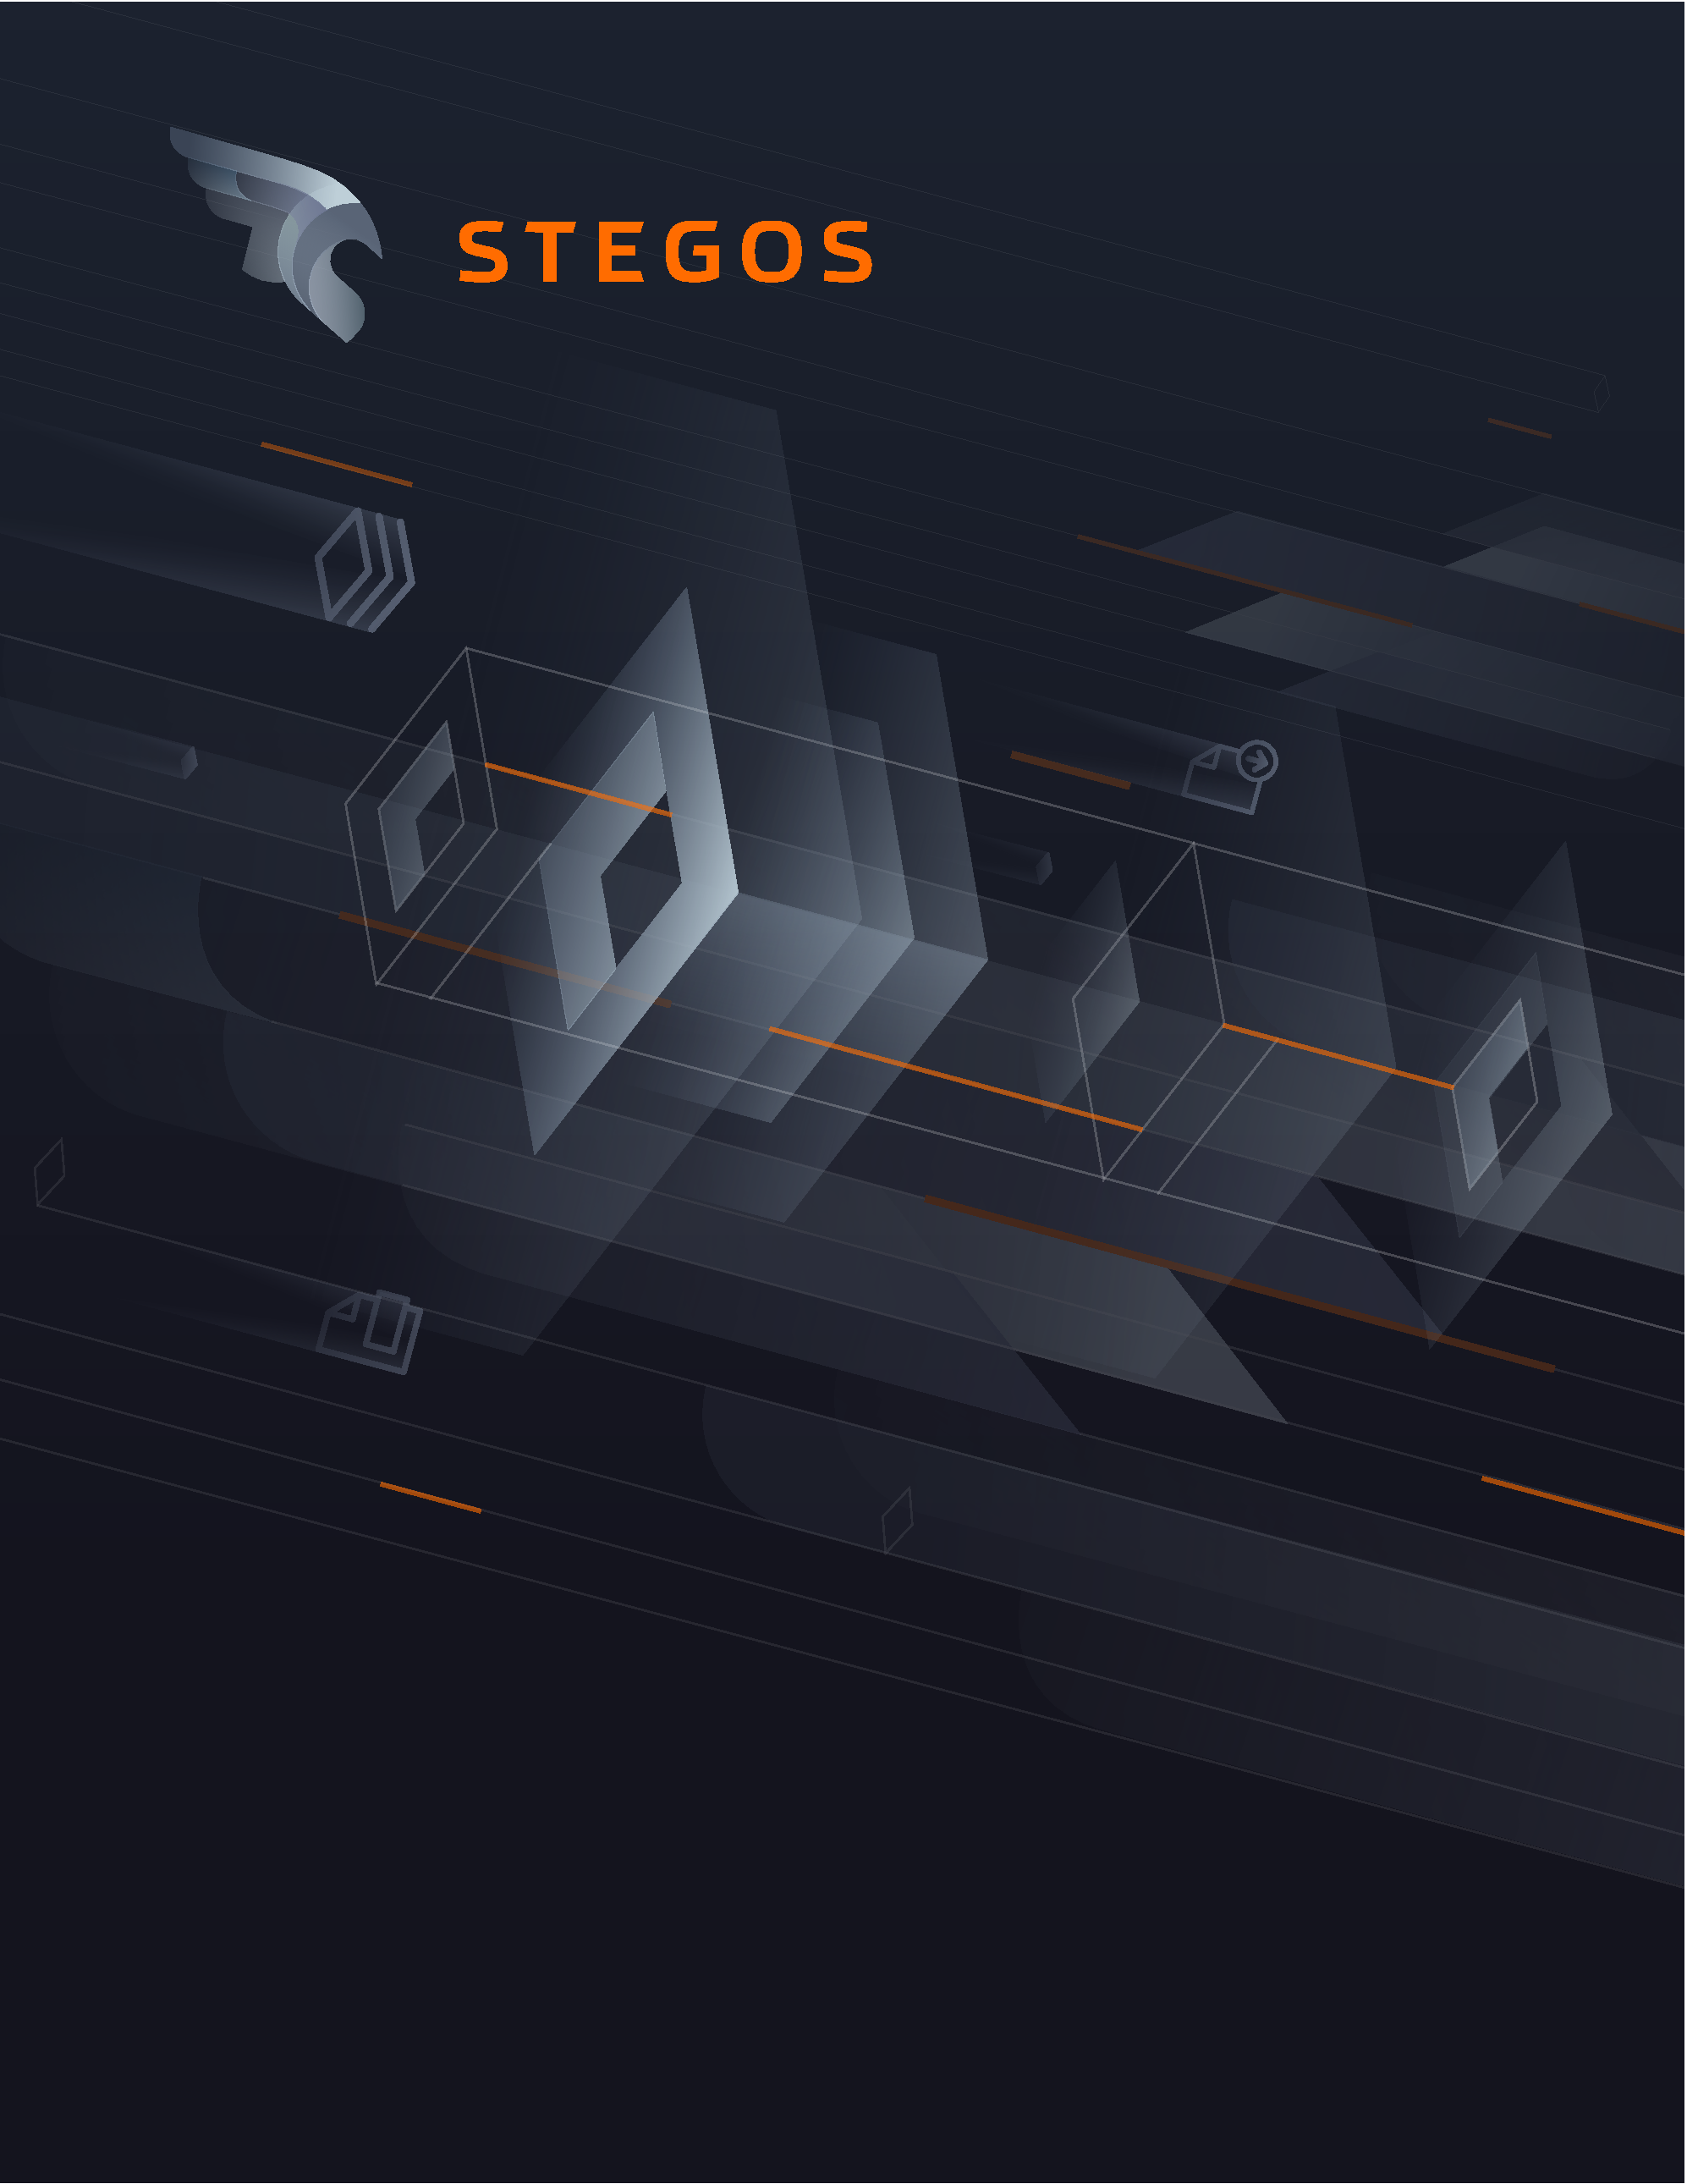
\includegraphics[width=\paperwidth,height=\paperheight]{images/front.pdf}}}
\maketitle
\endgroup

\nobreakspace

\vfill{\footnotesize\noindent{}Copyright \textcopyright\ 2019 Stegos AG\\
This work is licensed under a Creative Commons Attribution-ShareAlike 3.0
license (CC BY-SA 3.0).\\\\
All product names, logos, and brands used or cited in this document are
property of their respective owners. All company, product, and service names
used herein are for identification purposes only. Use of these names, logos,
and brands does not imply endorsement.}

\newpage

\tableofcontents\newpage

\section{Abstract}
Multipurpose mobile apps and social media platforms have allowed millions of previously unconnected people to access online services and communities. However, they do so at unacceptable costs to user privacy. Conversely, blockchain and cryptocurrency platforms offer unprecedented privacy benefits, but are currently unsustainably slow and resource-intensive, making them inaccessible to the average user. We need a way to marry privacy and accessibility in a single platform.

The Stegos Privacy Platform (Stegos) combines a unique blockchain and token design to implement the first cryptocurrency that’s completely private, secure, efficient, and environmentally sustainable. Stegos is fully scalable and prunable, ensuring the chain always remains compact without compromising trust. This makes Stegos the world’s first public blockchain to offer secure and confidential data storage and transmission in addition to payment transactions. 

Stegos extends this blockchain foundation to provide a platform for building privacy applications that communicate via messages sent with minimal latency. Our trusted application container (TAC) and privacy app store simplify the process of building and distributing privacy applications while providing additional security for users. Last but not least, Stegos marketplaces, chat, and red packets replicate the most popular features of modern multipurpose apps in a decentralized way, allowing users to transact and communicate in complete privacy.

Stegos is secured by the gamified Proof-of-stake (gPoS) consensus mechanism based on verifiably unbiased distributed randomness. gPoS allows anyone to run the Stegos blockchain from their pocket and earn tokens for maintaining the network, even without a high stake. This encourages an extremely wide user base by ensuring that mobile users are properly incentivized to validate the network.
\section{Feedback}

Please address comments and suggestions on this paper to \href{mailto:paper@stegos.com}{paper@stegos.com}.

\chapter{Introduction}\label{chap:intro}

\section{We All Deserve Privacy}
Everyone deserves privacy. They also deserve access to all the services and benefits of our modern digital world. But current technologies and business models are unable, or perhaps unwilling, to provide both simultaneously.

The past decade has seen the rise of global social media platforms and multipurpose apps with integrated payments such as WeChat and Facebook. This, combined with rapid advances in mobile internet and hardware, has allowed almost a billion people to get online and communicate, trade, and collaborate. But these platforms are a privacy nightmare: your every action can be tracked and linked to provide a full history of everyone you've ever communicated or transacted with, whether you want to share this information or not. In addition, user data is often harvested indiscriminately into enormous data silos, making them a target for unscrupulous advertisers, state actors, and hackers. Current efforts to curb this abuse are ineffectual and heavy-handed, often because governments and regulators are unwilling to cede control and let users take responsibility for their own online actions.

On the hardware side, solid-state technology, smartphones, and the Internet of Things let us carry our lives in our pockets, on our phones and on our laptops. But under the guise of protecting us — from terrorism, from hackers, from our own alleged lack of responsibility — our privacy has been decimated. In airports, online, even on the street, we are forced to reveal our private data with alarming frequency.

This intrusion leaves many of us feeling exposed and powerless. Many face even more chilling consequences, such as the loss of their jobs, liberty, or even lives. 

We live in an era of unprecedented state surveillance and crackdowns on freedom of the press and even thought. It’s nobody’s business what you do with your money, whether paper or digital, and it’s nobody's business who you transact with on the blockchain.

These trends have not gone unnoticed. Across the world, people are voicing their displeasure at how their privacy and data are being exploited for profit. There is a groundswell of demand for more secure and private alternatives, and this is only going to grow over the coming months and years.

\section{Blockchain and Privacy}
At the other end of the spectrum, blockchain and decentralized technologies have facilitated massive leaps forward in digital privacy and security. While traditional data sharing and storage technologies (online cloud storage, email, laptops, etc.) have built-in security, these technologies can easily be compromised. Once someone obtains and enters your password, your data is permanently exposed.

A private decentralized solution based on blockchain is a far better way to keep your private information safe and share it with people you trust.

However, adoption levels have been disappointing. Current blockchains are slow, unwieldy, and environmentally disastrous, and no privacy coin is as private as it claims to be. The reliance on resource-hungry static hardware and unfriendly interfaces puts this technology beyond the reach of regular users, without whom blockchain platforms are doomed to wither and recentralize. As users in all walks of online life increasingly migrate from desktop to mobile, crypto is failing to keep pace. 

The solution is clear: In order to thrive, blockchain platforms must emulate the mass appeal and usability of platforms such as WeChat and Facebook while maintaining strong privacy, anonymity, and decentralization.

Stegos is the first blockchain to combine these worlds. Stegos is the best mechanism for secure transactions, data transmission, and communications because, unlike traditional email and online messaging services, it’s completely decentralized, cryptographically secure, and leaves no telltale clues to user identity. It’s impossible to see who sends or receives information or establish how anyone is connecting to Stegos. No-one but the intended recipient of a communication or transaction can see what or how much was sent, and there’s nothing to link data or transactions to anyone’s real-life identities.

Stegos is also the first blockchain that's truly mobile compatible: smartphone nodes have full validation capabilities and there's no hardware-intensive Proof-of-work, meaning anyone can earn coins for supporting the network. By giving data transmission and messaging the same priority as regular transactions, Stegos is a platform that people will actually want to use. And the focus on smartphones means people will actually be able to use it.

In our modern connected world, everyone should have access to secure and private transactions and communications. Stegos is the first and only blockchain platform that can provide this.  

\chapter{What is Stegos?}\label{chap:what-is-stegos}

\section{Summary}
The Stegos Privacy Platform (Stegos) combines a unique blockchain and token design to implement the first cryptocurrency that’s absolutely private, secure, efficient and environmentally sustainable. Stegos uses the \textit{UTXO} (coin) model and \textit{gPoS} (gamified Proof-of-stake) consensus, combining existing privacy coin ideas and the latest cryptographic research to create a fully scalable and prunable privacy blockchain and application platform. 

\subsection{Absolute privacy}
Payment and data transactions in Stegos are unlinkable, untraceable, and completely confidential thanks to Stegos' Snowball protocol (see Appendix \ref{app:snowball}). Every Stegos transaction is directed to a new and unique stealth address, making it impossible to identify the recipients. Snowball also makes it impossible to trace Stegos transaction history, since individual transactions are first joined together to form a supertransaction before being submitted to blockchain validators. This is all done in a secure and privacy-preserving way, while ensuring that Stegos coins remain fully fungible.

\subsection{Payments and messaging}
Other privacy tokens — such as Monero, Dash, ZCash, and Grin — can only be used for payments, and all display weaknesses in terms of scalability, privacy, security, or usability. Stegos builds and improves upon these and other privacy coins and can be used to send both payments and data with complete confidentiality. The Stegos trusted application container (TAC) allows developers to easily build applications that communicate anonymously, privately, and efficiently.

\subsection{Scalability and data compaction}
Stegos is a fast and highly scalable blockchain and, unlike other blockchains, it's kept small without compromising trust. Details of spent coins and consumed data are safely removed from the blockchain using secure cryptographic pruning. It's also highly scalable thanks to transactional sharding. This makes Stegos the world's first public blockchain that can offer secure and confidential data storage and transmission in addition to payment transactions. It also ensures that Stegos is compact enough to run on smartphones.

\subsection{Proof-of-stake (PoS)}
Stegos is environmentally friendly and does not waste megawatts of electricity mining blocks. Instead, Stegos uses a bespoke gamified Proof-of-stake (gPoS) consensus, building on advancements in distributed systems theory and cryptography. Each new Stegos block must be verified and confirmed by a group of validators, all of whom must post tokens as bonds. The value of the tokens staked in this way directly affects the probability that a validator will win a block and earn the associated transaction fees.

\subsection{Mobile app}
To showcase the power of the platform, Stegos is developing its own native multi-purpose mobile application that integrates a wallet, one-one-one and group chat, the TAC, the Privacy App Store and the Stegos red packets \ref{sec:red-packets}. This app will be the gateway for users onto the Stegos Privacy Platform.
	
%% Overview

\section{Private by Default}
The original Bitcoin paper only included a very small section on privacy\cite{c1}. It assumed that even though transaction amounts are public, it would be impossible to link those transactions to anyone’s real identities. This assumption has repeatedly been proven wrong by researchers, blockchain analysis companies, and hackers. Software like ChainAnalysis has made transaction analysis trivial, allowing anyone to quickly de-anonymize users of Bitcoin and other cryptocurrencies.

Most blockchains have followed in Bitcoin’s footsteps with a totally transparent design that includes visible addresses and amounts, including the balance of any wallet, how much money has been sent and received, and the addresses of every sender and recipient. But all this readily available information paints a large and highly visible target for hackers and Big Brother. With the rise of privacy technologies like Bulletproofs and zk-SNARKs, there’s no excuse to perpetuate Bitcoin’s mistake. Blockchain should be private by default.
	
To this end, transactions in Stegos are \textit{unlinkable}, \textit{untraceable}, and \textit{confidential}:

\begin{itemize}
	\item Stegos uses one-time payment addresses which make it impossible to identify recipients of a transaction. Our technique for one-time addresses is very similar to the stealth addresses used in Monero and ZCash.
	\item Stegos pools individual transactions to form super-transactions, making it impossible to trace transaction histories. For this purpose, we have developed an improved version of the ValueShuffle protocol\cite{c7}, the first coin mixing protocol compatible with confidential transactions.
	\item All amounts in Stegos are hidden using Pedersen commitments\cite{c8} and Bulletproofs (range proofs)\cite{c4}. Validator stakes and transaction fees are the only exception, since these must be visible for blockchain validation.\end{itemize}

We call the combination of these privacy features Snowball (for more detailed information, see Appendix \ref{app:snowball}). %Is this right?

\section{Gamified Proof-of-stake (gPoS) consensus}

Standard Proof-of-stake consensus can leave many users with smaller stakes unincentivized. To address this, Stegos employs \textit{gamified Proof-of-stake} (gPoS), so-called because every validator which has been running for a certain amount of time has the chance to receive a random \textit{Validator service award}, regardless of the size of their stake\footnotemark.

\footnotetext{A nominal minimum threshold will apply to prevent users from gaming the system, but since every eligible node must provide validation services to qualify, it is impossible to spam the system, as one goal of the \textit{Validator service award} is to maximize the number of different nodes.}

To fund this, a portion of the reward from each block is added to the service award pool, which continues to grow until a winner is selected in an ongoing \textit{cryptographic lottery} based on verifiable distributed randomness. 

Because smartphone nodes can have full validation capabilities, anyone can earn tokens from their pocket.

\section{Sharding for scalability}
Stegos uses transactional \textit{sharding} to scale. Separate groups of Stegos validators keep the whole blockchain state but verify only a subset of incoming transactions, using cross-shard atomic commits to eliminate double-spending. This scalability approach allows Stegos to process thousands of transactions per second across millions of mobile devices, making Stegos the first and only blockchain that can run entirely in your pocket. 

\section{Pruning and data compaction}
Many projects claim to be able to process hundred of thousands or even millions of transactions per second (tps), but few explain how they plan to maintain all the accumulated data. Even at its paltry 7--10 tps, the Bitcoin blockchain is now larger than 200 gigabytes. Assuming Bitcoin could suddenly support 16,000 tps, the Bitcoin blockchain would grow by 350 gigabytes every day\footnote{https://hackernoon.com/if-we-lived-in-a-bitcoin-future-how-big-would-the-blockchain-have-to-be-bd07b282416f}, or 127 terabytes every year. This amount of data is completely unsustainable without the blockchain being centralized on a few supercomputers, which runs contrary to the decentralization ethos of blockchain.

Stegos is a \textit{compact} blockchain. Spent coins and expired data are safely removed from the blockchain using secure cryptographic pruning. To keep our blockchain free of spent coins, we use the technique proposed by Satoshi Nakamoto in the original Bitcoin paper\cite{c1}. Data is removed quickly and automatically.

\section{Fast data messaging}
Unlike other blockchains, Stegos does not restrict users to sending just payments. Stegos supports data messaging, allowing users to exchange data messages with the same privacy guarantees afforded to payments. Data is a first-class citizen on the Stegos blockchain, which is only logical as the average user is expected to send many more data messages than standard payments.

\section{Stegos mobile app}
The Stegos mobile app is the portal into the Stegos ecosystem and a showcase of the potential of our platform. The app integrates a wallet with a secure environment for running privacy-focused applications. In this way, Stegos can provide all the functionality of existing centralized multipurpose apps such as WeChat, but in a fully private and decentralized manner. 

Features include one-on-one and group chat facilitated by the Stegos fast message bus, integrated payments and red packets, an extremely popular WeChat feature that allows anyone to send a hongbao-style surprise payment to a specific user or group of users or to create a custom token airdrop that anyone can claim by scanning a QR code.

The Stegos app also gives users simple and direct control of their staking, making it easy for everyone to participate in maintaining the network. 

Everyone deserves privacy. And everyone should be rewarded for contributing to a more private world. Stegos doesn't just keep your money and secrets safe. It rewards you for maintaining the network, even on your phone.

\section{Privacy applications}
Stegos is committed to meeting the growing demand for privacy and data security without sacrificing usability or accessibility. Research shows that millions of users are dissatisfied with platforms such as Facebook and WeChat, but without a functionally equivalent alternative they feel locked in and unable to switch. To meet this need, Stegos is designed to encourage a blooming ecosystem of privacy applications, with Stegos messaging acting as a secure and private message bus between them.      

\subsection{Trusted application container (TAC)}
Accessibility and usability are not solely user requirements. Developers also need to be catered to if they are going to switch to developing to a new platform. Developing native mobile applications is hard and error-prone. Developing secure mobile applications is harder still, and blockchain only adds an extra level of difficulty. Stegos aims to make developing mobile privacy applications simple and painless while protecting users from malicious or badly written applications. 

The Stegos \textit{trusted application container} (TAC) is a native mobile application and a container for deploying privacy applications. Applications can be built using familiar technologies like Javascript, HTML, and CSS and run as plugins in a \textit{sandbox}, with tightly controlled access to the user’s wallet and the outside world.

\subsection{App Store}
Users need a way to easily discover and install applications. The Stegos Privacy App Store will provide an on-chain mechanism to search and install privacy applications, developed to run in the TAC, as well as rate their usefulness.  

\section{Private marketplaces}
Private transactions aren't just limited to token payments. While transferring tokens is an extremely important use case for many users (e.g., remittances), most transactions involve payment for some kind of tangible goods or services. By combining private payments, fast messages, chat, and the TAC, Stegos can deliver private marketplaces where items can be sold anonymously and privately. 

Stegos will release a separate mobile app as the marketplaces interface.  

\section{Incentives to drive adoption}
Decentralized networks draw strength from the breadth and engagement of their user base. To encourage widespread adoption, Stegos includes various incentives aimed at a variety of different user groups. 

In addition to standard staking payouts which reward validators in proportion to their stake, the \textit{Validator service award} is a unique Stegos feature that rewards validators simply for being online and helping support the network. A third of the tokens from each block reward are added to the service award pool,\footnote{Along with any tokens from expired red packets.} which is then distributed every few thousand blocks. Validators run a \textit{cryptographic lottery} based on verifiable distributed randomness to select a single validator to receive the award. The current size of the service award pool is visible to all users via the Stegos app.

\textit{Red packets}\footnote{https://en.m.wikipedia.org/wiki/Red\_envelope\#Digital\_red\_envelopes} are based on a wildly popular WeChat feature which is in turn based on the Chinese tradition of hongbao. The introduction of the Red Packet feature encouraged millions more users to sign up to WeChat, including revealing their personal banking details. Stegos intends to replicate the popularity of this feature without invading user privacy.

Like their centralized equivalent, Stegos red packets come in various flavours: they can be public or private, and the amounts inside can be fixed or randomized. In the simplest form, a red packet can be used to send a fixed amount of tokens to another user or group of users via Stegos chat. The amount is a surprise, and will not be revealed until the user opens the packet.

Red packets in private group chat can also be randomized, with every group member receiving a random prize. 

Stegos also allows user to create public red packets, a feature designed to disseminate tokens and promote awareness, both for Stegos itself and for individual privacy apps and private marketplaces within the Stegos Privacy Platform. Public red packets are similar to airdrops, but encourage more active participation among a wider pool of users. 

Anyone can create a public red packet and fill it with a number of tokens of their choice. They should then distribute the corresponding QR code or URL to the target audience. Each attempt to open a red packet may result in randomly determined token prize. Prizes are awarded until the packet is empty or a day has passed, at which point any unclaimed tokens will be added to the validator service award pool.

More information about the implementation of Stegos red packets can be found in Section \ref{sec:red-packets}.

\chapter{Privacy applications platform}\label{chap:privacy-app-platform}
The Stegos Privacy Platform builds on top of our fast message bus (Section \ref{sec:fastdata}) and makes developing mobile privacy apps a breeze. The Stegos mobile app is the primary window to the platform. It integrates the trusted application container (TAC) with one-on-one and group chat as well as the Privacy App Store and red packet feature. 

\section{Trusted Application Container}\label{sec:tac}
The Trusted Application Container (TAC) is a sandbox and virtual machine (VM) for running plug-in apps written using HTML, CSS and JavaScript. The architecture is very similar to that of WeChat mini-programs \footnote{https://walkthechat.com/wechat-mini-programs-simple-introduction/}.

The TAC prevents apps from wreaking havoc on the host phone. It also completely abstracts the blockchain from running applications, instead providing an interface (API) to send messages and access the wallet. The TAC tightly controls access to the outside world and ensures that spending tokens requires confirmation from the user. 

Stegos will provide a software development kit (SDK) and documentation for building privacy apps. 

\section{Identity}\label{sec:identity}
Every Stegos wallet has a public key (address) associated with it. Stegos uses \textit{stealth addresses}, and payments to a public key are cloaked with two random values. This makes it impossible to link payments to someone by analyzing the blockchain. Only the sender and the receiver are privy to any exchange of information. This means users do not have to be overly protective of their public key: it’s completely safe to post a Stegos public key on a website or even plaster it on a street billboard. 

Stegos uses the unspent transaction (UTXO) model, where each UTXO is best understood as a coin. There’s no separate notion of identity in Stegos, although wallet addresses can be used as an identifier or avatar for the purposes of messaging or building a reputation or social score on Stegos private marketplaces or other privacy applications. 

Stegos users can export their wallet address as a QR code.

\section{Privacy App Store}\label{sec:appstore}
Users have different privacy needs, and sometimes even knowing that a user has a particular app can risk a privacy breach. Users need a way to privately browse and access apps, while being confident that the apps they install are private and secure. To achieve this, Stegos implements an on-chain privacy app store, where details of the apps are stored on the Stegos blockchain itself.

The apps themselves should be stored off chain to avoid bloating the Stegos chain, but to be listed on the Stegos privacy app store, each privacy app must create a manifest which includes a description of the app, the URL used to download it, and a hash of the app bundle. This manifest is stored on the Stegos blockchain. App bundles are signed with the developers' public key, which allows users to leave on-chain app reviews to rank individual apps and developers. Manifests also contain tags to allow users to search the app store by category.

Apps are downloaded via the Stegos app. Once downloaded, the TAC verifies that the signature of the app bundle and the hash match the information in the manifest. The TAC installs the app bundle locally and makes the app available in the Stegos mobile app. Users can delete apps at any time.

\section{Chat}\label{sec:chat}
No matter how well a blockchain obscures user information in its transactions, users still need a way to find each other, which risks exposing their personal information. This affects some coins more than others. MimbleWimble, for example, requires users to communicate in advance to share the blinding factors needed to obfuscate identifying details about their transaction. But every transaction requires some initial communication between parties in order to define the parameters of the trade. If this communication can be intercepted, malicious third parties can begin deanonymizing a coin’s transaction history. 

Existing platforms generally leave this problem to users to solve, drastically reducing their appeal and effectiveness. While information leaks can never be fully plugged, at Stegos we believe it is the responsibility of the platform to provide users with as many tools as possible to protect their privacy. Every transaction which can be protected in this way increases the privacy of all users across the platform.

To this end, Stegos implements fully private communication and integrates it within the Stegos app. It functions like a standard messaging app which all users will be familiar with. Users use their public keys as an identifier (Section \ref{sec:identity}), safe in the knowledge that this can be exposed without revealing any links to other users or transactions. Messages are transmitted via the fast message bus (Section \ref{sec:fastdata}), ensuring that messages are received almost instantly.

Users can send a QR code via private chat to initiate an STG transaction. It is also possible to create chat groups and invite people to chats via QR codes. 

In the following chapters we explain the Stegos features in more detail.

\chapter{Stegos in depth}\label{chap:stegos-in-depth}

\section{Consensus}
The Stegos consensus protocol is based on \textit{Albatross}\cite{c23}, a novel blockchain consensus algorithm inspired by speculative BFT\cite{c9} algorithms, and has strong consistency while often achieving instant transaction confirmation. The Stegos consensus protocol is secure and has a performance close to the theoretical maximum for a single-chain PoS consensus algorithm.

\subsection{Speculative BFT}
Speculative BFT algorithms that have two modes for consensus: 

\begin{enumerate}
	\item the \textit{optimistic mode}, where speed is preferred and few security measures are applied, under the assumption that the nodes are well-behaved, and
	\item the \textit{pessimistic mode}, where the only goal is to make progress even in the presence of malicious nodes.
\end{enumerate}

The optimistic mode allows the Stegos consensus protocol to compete for speed with centralized systems. Nodes verify each update and when an invalid updated is detected, consensus switches to pessimistic mode. The invalid update is discarded and then consensus reverts to optimistic mode.

\subsection{Validators}
Stegos is a public ledger, so anyone can join the network, become a validator, and earn rewards for maintaining the blockchain. Stegos uses gamified Proof-of-stake (gPoS) consensus to better incentivize smaller stakers compared to standard Proof-of-stake. Nodes need to post a performance bond (stake) to be eligible to provide validation services. Requiring a performance bond protects against Sybil attacks by requiring a financial commitment from validators. Locked tokens can be staked just like regular ones.

Validators who have posted a performance bond are eligible to be randomly selected to participate in a consensus round as an active validator. Individual active validators are selected to create blocks using verifiable distributed randomess and are rewarded with the block reward and transaction fees from the blocks they sign. The other active validators witness and cosign the created blocks, making them eligible for the validator service award (Section \ref{sec:service-award}).  

\subsection{Blocks}\label{sec:blocks}
Stegos has two types of blocks:

\begin{itemize}
	\item {\em Key blocks} Key blocks are used to change the validator list and act as checkpoints in the Stegos chain. Key blocks only contain the identities of the new subset of active validators and the random seed used to select them. Key blocks are produced with pBFT and cannot be forked.
	\item {\em Regular blocks} Each regular block is produced by a verifiably randomly chosen active validator and contains not only the user transactions to be included, but also the current state and a random seed produced by the validator. These blocks are produced optimistically and only need to be signed by the corresponding validator.
\end{itemize}

One key block is always followed by a fixed number of regular blocks. An \textit{epoch} is composed of a key block and the regular blocks that precede it. Every epoch, the list of validators is updated and a new list of active validators is randomly selected.

\subsubsection{Block frequency}
Under test conditions and assuming a $16$-node network, we observed a block propagation time of $500ms$ - $700ms$. We expect this number to be higher in practice, but still within $5s$ for a regular block. 

Key blocks involve pBFT consensus and thus take longer to create. In testing, we observed times of around $5s$ for $16$ validators. The number of validators will be much larger in practice, but we still expect a key block frequency in the range of $30s$ to $60s$.

A key block frequency of $2min$ should ensure that the ratio between the number of key blocks and regular blocks is sufficient to capitalize on the optimistic mode without compromising security.

\subsection{Validator Selection}
Validators are selected from the active validator pool using a stake-weighted lottery. The larger the validator’s stake, the greater their chance of becoming the pBFT leader (when creating a key block) or being selected as slot owner (when creating a regular block).

\subsection{Fork resolution}
Validators will choose the longest chain, i.e., the chain with the most blocks, as the main chain. Because key blocks require pBFT consensus, forks can only occur between two key blocks. Therefore, nodes only need to consider chains that include the latest key block.

We apply the following heuristics from top to bottom to resolve a fork:

\begin{enumerate}
	\item The chain with the most key blocks.
	\item The chain with the blocks with the highest pBFT view change number.
	\item The chain with the most blocks.
\end{enumerate}

In case of a tie on all three conditions, the next validator can build on top of either chain.

\subsection{Punishing misbehaving validators}
There are three ways a validator can misbehave in our consensus implementation: producing an invalid block, creating a fork, and delaying a block. These nead to be dealt with and disincentivized where appropriate.

We deal with the three types of misbehaviour as follows:

\begin{enumerate}
	\item {\em Invalid blocks} - When a validator produces an invalid block, the other validators will ignore that block. Validators will also ignore any more blocks from that validator during the current slot, which helps prevent DoS attacks.
	\item {\em Forks} - Forks are not possible during a key block, because pBFT is a forkless protocol. But a fork can be created if a validator produces more than one regular block in the same slot. In this case, both forks are ignored and a new active validator is selected using the pBFT view change protocol. 
	\item {\em Delays} - Validators can too long to produce a block, or can go offline entirely. In both cases, we change the slot owner using the pBFT view change protocol. 
\end{enumerate}

To disenctivize these behaviours, we introduce \textit{slashing} to punish misbehaving validators. Slashing confiscates the stake of the validator who produced an invalid block or fork. The only proof needed for a fork is two block headers at the same slot signed by the same validator. The slashed stake is evenly distributed between the rest of the validators in the current epoch. Delays are not punished by slashing, because it is impossible to tell whether the delay was malicious or not, and we do not want to discourage mobile nodes, who are likely to have less stable connections.

\subsection{Collective Signing}
We adopt \textit{CoSi}\cite{c10,c11}, a scalable witness co-signing protocol ensuring that every authoritative statement is validated and publicly logged by a diverse group of witnesses before any client will accept it. A statement, $S$, collectively signed by $W$ witnesses assures clients that $S$ has been seen, and not immediately found erroneous, by those $W$ observers. 

Even if $S$ is compromised in a fashion not readily detectable by the witnesses, CoSi still guarantees $S$’s exposure to public scrutiny, forcing secrecy-minded attackers to risk that the compromise will soon be detected by one of the $W$ witnesses. 

CoSi builds on existing cryptographic multi-signature methods, scaling them to support thousands of witnesses via signature aggregation over efficient communications. The default implementation of CoSi uses Schnorr signatures which we replace with BLS signatures for performance reasons.

Active validators who participate in CoSi become eligible for the validator service award (Section \ref{sec:service-award})

\section{Networking}
The Stegos network is composed of three types of nodes: \textit{bootstrap nodes}, \textit{compact nodes}, and \textit{light wallets}. Bootstrap and compact nodes maintain a copy of the blockchain and associated data structures. After posting a performance bond (stake) to become \textit{validators}, these nodes participate in the consensus protocol and can earn block rewards and transaction fees. These nodes also respond to requests from light wallet nodes.

Bootstrap nodes carry the unpruned version of the blockchain and respond to bootstrap requests from new compact and bootstrap nodes. Compact nodes carry the pruned version of the blockchain, i.e., the current UTXO set. Light nodes only keep blockchain headers and know how to talk to validators. 

Stegos will initially maintain the core of the network by running a number of core bootstrap nodes to ensure network continuity and performance. The addresses of these core nodes will be hard-coded into each release of the Stegos blockchain software.

Nodes keep a list of addresses of the nodes they know about (peers) and add new peers to the list as they become aware of them. New nodes will connect to one of the core nodes to fetch a list of bootstrap nodes and download a copy of the blockchain. 

After a few light checks, each full node quickly rebroadcasts received transactions to a subset of its peers. This ensures that a node cannot be DDoS-ed with transactions to validate and that it does not rebroadcast junk transactions. To discourage bad actors here, we employ a mechanism to throttle peers and punish them for bad transactions, e.g., by blocking them from further participation in the network.

The Stegos blockchain uses a gossip protocol to spread information without depending on a fixed network topology. This protocol does not require every node to be reliable or always up and running, and does not require every node to know about every other node. Each node knows about just a few peers, and information can safely propagate through the network as long as most nodes know of at least two peers.

\section{Incentives}
Stegos is powered by the STG token, available once the mainnet is launched. When posted as a performance bond by nodes wishing to support the Stegos platform, the STG token gives validators the right to earn fees and block rewards when they are elected as the leader of the consensus round. The probability of a validator being elected the leader is proportional to the size of their stake.

\subsection{Validator service award}\label{sec:service-award}
Ledgers based on Proof-of-stake (PoS) can have difficulty maintaining a broad user base since most users have a vanishingly small chance of earning significant rewards. To mitigate this failing, gPoS includes a \textit{Validator service award} in addition to the standard block rewards and transaction fees. The award is meant to incentivize validators with small stakes to maintain the network. Instead of only allocating rewards to block creators, any node which has provided active validation services is eligible to win an award. This has an added effect of incentivizing witnessing of normal blocks and participation in the pBFT process for key blocks.

One third (1/3) of every block reward will be added to the service award pool, along with tokens from expired red packets. The validator service award is awarded to a single user, chosen from all users who have provided active validation since the last validator service award payout. The odds of the award being paid out starts small and increases with every block. Thus the precise time of the drawing cannot be predicted, but on average the validator service award will be distributed every 5-10 days. This frequency is chosen to ensure that most users who have posted a stake stand a good chance of becoming eligible, and that the reward should always grow large enough to be an appealing incentive to participate. 

\subsection{Red packets}\label{sec:red-packets}
Giveaways are one of the most popular and effective ways to increase participation and awareness of a platform. Since the launch of WeChat’s digital red packet function in 2014, millions of people have signed up to WeChat and voluntarily shared their bank details. The red packet app was responsible for more than 2 billion transactions on January 1st 2016 alone.

For cryptocurrency platforms, the most common form of giveaway is an airdrop. These are often a wasteful way to disseminate tokens, as the passive nature of airdrops does little to encourage participation, and their long-term effectiveness is unclear. While airdrops do seem to be an effective way to onboard community members, few of these make the jump to running nodes or actively using a platform.

To address these issues, Stegos implements a red packet feature similar to that seen on WeChat, but without the requirement for users to disclose personally identifying information. Red packets come in two forms: private and public. Private red packets can be used to send fixed amounts of tokens to a particular user or group of users. Public red packets are a gamified airdrop mechanism where the token payout is randomized.

Anyone with the Stegos app can create a red packet and load it with STG tokens. In addition to the number of tokens in the packet, users also choose the number of prizes which will be awarded (for a fixed surprise payment to a specific user, the number of prizes can be set at 1). The tokens are then randomly divided between different denomination coins (UTXOs) within the packet, with the number of coins equalling the number of chosen prizes. 

The app then generates a QR code or URL which can be used to access the red packet. On accessing the red packet, validators will randomly determine whether the user has won a prize or not. If they have, one of the remaining predetermined coin denominations will be transferred from the packet to the user’s STG wallet. This process continues until the red packet is empty or the expiry deadline passes.

Users can keep accessing a red packet until it is empty, although the network will enforce a small delay between attempts to prevent DDoS attacks. Accessing a red packet is free, and does not require users to buy tokens or pay transaction fees. However, a portion of all prizes will be awarded to validators as a processing fee.

Red packets expire after a day.  Because of the private nature of Stegos transactions, it is impossible to return unclaimed tokens to the user who originally set up the red packet. Therefore, any unclaimed tokens will be added to the validator service award pool.

Users must install the Stegos app and set up a STG wallet before they can open a red packet. With this barrier to entry crossed, users will be able to start running their own mobile validator node with minimal effort.

\section{Snowball}
\subsection{A problem of establishing untraceability}
Even though user identities are cloaked in the blockchain, the spending history of every UTXO can be established by tracing blockchain transactions backwards, up to the genesis block.

Despite having a serious hurdle for such tracing — we don’t store transactions in the blocks of out blockchain, but rather Merkle trees of inputs and outputs — a malicious node which joined the Stegos network immediately after mainnet release could theoretically collect all transaction histories in order to analyze and trace UTXOs.

To counteract this, Stegos will implement a protocol that completely hides the relationship between inputs and outputs of each transaction. This is difficult because UTXOs must have a unique $ID$, without which there would be no way to validate transactions or prove ownership of a UTXO. Unique UTXO IDs establish a trail which we want to obscure by only showing that UTXO output could have come from one of many different and unrelated inputs. We want to hide the source of each UTXO but in a manner that allows public validation.

\subsection{Possible solutions}
Currently there are four kinds of approaches to solving the problem of establishing untraceability: coin mixers, Ring Signatures, zk-SNARKs, and the CoinJoin family of protocols.

\subsubsection{Mixers} Mixers require users to trust the third party which provides mixing services, something that’s unacceptable in a truly private and confidential blockchain.

\subsubsection{Ring Signatures} Ring signatures collect a large but random number of existing UTXOs and add those into the list of inputs actually being spent. A signature is formed on all of the inputs, enabling proof that the inputs are properly spent as a group, without revealing the exact inputs being spent. 

Unfortunately, ring signatures prevent blockchain compaction since it’s impossible to know when a UTXO has been spent and prune it from the blockchain. All UTXOs \textit{that ever existed} must be retained, which is impossible to adequately scale.

\subsubsection{zk-SNARKs} zk-SNARK stands for ``zero-knowledge succinct non-interactive argument of knowledge.’’ Currently, the only known way to produce non-interactive zero-knowledge proofs that are short enough to publish to a blockchain is with an initial setup phase that generates a common reference string shared between prover and verifier. Anyone with access to the secret randomness used to generate this string can create false proofs that will appear valid to the verifier. For a cryptocurrency that uses zk-SNARKs, e.g., Zcash, this means the ability to create counterfeit coins. 

To prevent double-spending in a zk-SNARK-based cryptocurrency, nodes must maintain a cryptographic accumulator containing the serial numbers of all spent coins. This accumulator always grows and cannot be trimmed, which prevents adequate scaling.

\subsubsection{CoinJoin} is a protocol for joining several Bitcoin transactions together before submitting them to miners to include in the block. The protocol was originally proposed by Greg Maxwell in 2013 and is based on the following idea: ``When you want to make a payment, find someone else who also wants to make a payment and make a joint payment together.’’\footnote{https://en.wikipedia.org/wiki/CoinJoin} CoinJoin implementations are based on the use of trusted servers that mix multiple transactions together, which introduces an unacceptable level of trust to the system.

Each of these existing approaches introduces unacceptable processing costs or required trust. Most of these are unresolvable. However, the CoinJoin approach can be improved to resolve its trust issues. In 2014, CoinJoin inspired researchers from Saarland University to develop a completely decentralized protocol they called \textit{CoinShuffle}\cite{c17}. It also allows users to mix their coins with those of other interested users and uses the accountable anonymous group communication protocol \textit{Dissent} to ensure anonymity and robustness against DoS attacks. 

The same researchers presented an enhanced version of the protocol in 2016, which they called \textit{CoinShuffle++}\cite{c18}. The key innovation of CoinShuffle++ is to replace mix-nets with Dining Cryptographers Networks (DC-nets)\cite{c20}, a more efficient anonymity mechanism. 

A mix-net requires sequential processing so the number of communication rounds in the original CoinShuffle protocol grows linearly with the number of users. By using DC-nets, CoinShuffle++ allows for mixing to proceed in parallel, requiring a constant number of communication rounds regardless of the number of users.

Stegos adopts the CoinShuffle++ approach but improves it still further.

\subsection{ValueShuffle}
\textit{ValueShuffle}\cite{c19} is an extension of CoinShuffle++ that is compatible with confidential transactions. ValueShuffle ensures the anonymity of mixing participants as well as the confidentiality of their payment values, even against malicious mixing participants. Stegos adopts this approach, while improving and completing it in several key areas. First, the ValueShuffle paper is missing some key details: For example, the paper provides no details on how to form a pool of senders who wish to mix their transactions, nor how to form a signature on the resulting pooled transaction. 

We implement a protocol where a \textit{facilitator} elected among the validators provides the services of the \textit{Bulletin Board} (as defined in the ValueShuffle protocol). We also implement collective Schnorr signatures\cite{c22} on the resulting transaction. Details of these protocols, as well as a brief explanation of our implementation of ValueShuffle, are given in Appendix \ref{app:snowball}.

\section{BlockCrunch}\label{sec:pruning}
BlockCrunch is the Stegos algorithm for pruning the blockchain and keeping it compact. As described in Section \ref{sec:blocks}, a regular Stegos block is composed of a header and a body, where the header contains root hashes of the two Merkle trees that comprise the body of the block. These two trees are a tree of all inputs (\textit{TXIN} Merkle tree) and a tree of all outputs (\textit{TXOUT} Merkle tree). 

When a new block is verified and signed, the signature is computed over the block header alone. The body of the block does not need to be signed because it is secured against modification by the nature of the Merkle tree. That is, it will be impossible to modify the body of the block without invalidating the root hashes contained in the signed header.

Stegos blockchain compaction is a continuous process where each incoming and properly signed block triggers the pruning. As a result of this continuous pruning, the Stegos blockchain becomes a database of unspent coins (UTXO), with no transaction history kept.

After verifying and signing a new block, the \textit{leader} broadcasts it to the network. All nodes must validate the collective block signature and process the new block using the following steps:

A node must perform the following pruning algorithm for every regular block:

\begin{algorithm}
\begin{algorithmic}
	\State $block \gets <This Block>$
	\State $tree \gets \Call{Get-TXIN-Merkle-Tree}{block}$
	\State $leaves \gets \Call{Merkle-Tree-Leaves}{tree}$
	\For{$leaf \gets leaves$}
	\State $id \gets \Call{UTXO-ID}{leaf}$
	\State $block’ \gets \Call{Find-Block-With}{id}$
	\State $tree’ \gets \Call{Get-TXOUT-Merkle-Tree}{block’}$
	\State $leaf’ \gets \Call{Find-Leaf}{tree’, id}$
	\State \Call{Mark-As-Spent}{$leaf’$} \Comment{Does not touch the hash of the leaf}
	\For {$sibling \gets \Call{Get-Sibling}{leaf’}, \Call{Is-Spent}{sibling$}}
		\State $parent \gets \Call{Get-Parent}{leaf’}$
		\State \Call{Mark-As-Spent}{$parent$}
		\State \Call{Delete-Node}{$leaf’$} \Comment{Removes the hash}
		\State \Call{Delete-Node}{$sibling$}
		\State $leaf’ \gets parent$
	\EndFor
\EndFor
	
\If {$\Call{Is-Empty}{tree}$}
	\State $\Call{Delete-Tree}{block, tree}$ \Comment{Leaves just the hash in the block header}
\EndIf
		
\end{algorithmic}
\caption{Pruning algorithm}
\label{code:pruning}
\end{algorithm}

\section{FastData}\label{sec:fastdata}
Stegos introduces data transactions in addition to regular payment transactions. Both types of transactions enjoy the same encryption and privacy protection. In fact, because data is sent using zero-value coins, there’s no way to tell payments apart from data messages. 

Data messages are meant to be handled at the application layer and the payload is expected to include a sequence number. Unlike payments, data cannot be double-spent, so there’s no need to wait for data messages to become irreversible. The message sequence number should help applications order messages and check for messages that are missing. 

Stegos data messaging is a lot like UDP/IP and serves as a message bus that all kinds of applications can use to communicate securely and privately.

Data messages are automatically recycled and removed from the blockchain using BlockCrunch (Appendix \ref{sec:pruning}).

\chapter{Future work}\label{chap:future-work}

\section{Mobile staking}\label{sec:mobile-staking}
Mobile staking will not be available on the launch of the mainnet. However, we are making it a priority to implement mobile staking as soon as possible. Mobile staking will drastically increases the number of validator nodes, increasing the resilience and throughput of the network. Combined with ePoS, this will help prevent the stagnation and centralization witnessed by many blockchain projects.

\section{Marketplaces}\label{sec:marketplaces}
Fully private token transactions are extremely useful, but on their own they only provide a part of the necessary functionality for private transactions, most of which involve an exchange of goods and services. Being able to transfer tokens privately is only of limited use if the rest of the business of the transaction cannot be obfuscated. Currently, most privacy platforms leave this problem up to the user to solve, drastically reducing their usability.

By building on the features described so far, Stegos private marketplaces provide all the necessary tools to sell goods and services and even operate entire stores in complete privacy.

Vendors set up storefronts as mini-apps in the TAC, using their wallet public key as an identifies. An API will allow vendors to update their inventory. Using the same manifest system described for privacy apps (Section \ref{sec:appstore}), users can browse for particular stores and verify the storefront via the vendor’s public key signature. Users will access Stegos marketplaces via a separate marketplace app. Buyers and sellers can message each other using the Stegos chat service (Section \ref{sec:chat}). 

Private marketplaces use a form of hashlock (TBD) to atomically swap a payment for the item’s description key. The swap will only occur once both parties are satisfied with the terms of the transaction.

\subsection{Reputation}
Online marketplaces often rely on a ranking and reputation system to allow buyers to determine which vendors are trustworthy (and vice versa). Stegos supports this feature by allowing users to upload reviews and ratings to the blockchain, signed with their public key. When searching for a vendor via the marketplace app, reviews and ratings will be parsed from the chain and aggregated, allowing buyers to see a verified overall ranking for each vendor.

Unfortunately, anything which links transactions together is a potential privacy risk, so users must weigh the benefits against the risks depending on their own privacy requirements. As such, participation in the reputation system is entirely optional for vendors.

\section{Roadmap}\label{sec:roadmap}

\begin{table}[ht]
\centering
	\begin{tabular}{@{\extracolsep{4pt}}lll}
	\toprule[2pt] 
	Year & Target date & Deliverable \\
	\midrule[2pt]
	2019 & 31.05 & Mainnet and native token\\
	{} & {} & Cross-platform node UI \& wallet \\
	{} & Q3 & Exchange token sale \\
	{} & {} & Mobile app \\
	{} & {} & Dandelion \\
	{} & Q4 & Sharding \\
	{} & {} & Mobile (compact) node \\
	{} & {} & Mobile staking \\
	2020 & Q1 & App Store \\
	{} & {} & Private marketplaces \\
	{} & Q2 & Pruning with no bootstrap nodes \\
	{} & {} & zk-STARKs \\
	\bottomrule[2pt]
	\end{tabular}
\caption{Roadmap} 
\end{table}

The Stegos team is currently working on implementing the blockchain. The development progress can be tracked on \href{https://github.com/orgs/stegos/projects/1}{GitHub}. Our platform source code is and always be 100\% open.

\section{Conclusion}
This paper laid out a design for Stegos \textemdash a private, confidential, and scalable blockchain which is environmentally sustainable and optimized for storing and transmitting both data and payments.

Other privacy projects view privacy as a trade-off: requiring users to accept a slower, bloated, more resource-intensive blockchain in exchange for (questionable) privacy improvements. They also give little thought to the context surrounding transactions, leaving users to work out how to privately communicate and coordinate the terms of their trade. 

Stegos is different. Stegos combines the best developments in privacy technology with mechanisms for a faster and more scalable blockchain \textemdash along with plenty of innovations of our own \textemdash to create a blockchain where the privacy features make the blockchain more efficient, not less.        

By aggressively pruning the blockchain, Stegos is able to support a wide variety of on-chain features beyond simple token transfers. By combining chat, an on-chain app store and a trusted application container (TAC), Stegos facilitates every part of a fully private exchange of goods and services, not just the final payment step.

Stegos uses verifiably unbiased distributed randomness and a gamified Proof-of-stake consensus mechanism to create the first truly mobile blockchain. By embracing smartphones and providing an integrated app as a gateway to the platform, Stegos intends to be the first truly accessible blockchain, giving everyone easy access to the privacy they deserve.     

\chapter{Team}\label{app:team}

The Stegos team doesn’t just bring blockchain experience to the table (although we have plenty of that, too). With backgrounds in finance, aerospace, and cryptography, the team has a breadth of experience in applying technology to some of the most sensitive challenges facing society.

\section{Joel Reymont CEO, The Buck Stops With Me!}

{
\setlength\intextsep{0pt}
\begin{wrapfigure}{l}{0pt}
	
\includegraphics{images/team/team-1.png}
\end{wrapfigure}

Joel is a seasoned hacker and blockchain pioneer. He started his career on Wall Street and brings twenty-five years of diverse software engineering and management experience to Stegos. Joel was previously Chief Technology Officer at a Top 100 cryptocurrency and blockchain company, where he earned a reputation within the community for his formidable ability to get things done. Joel has acted as Director of Prime Brokerage Technology at Deutsche Bank, has run offshore development teams, and has built many scalable and fault-tolerant systems over the years. He now smashes technological boundaries and ventures deep into the unexplored frontiers of crypto to bring unique opportunities to Stegos contributors. 

Joel does not use social networks but has a very active \href{http://twitter.com/joelreymont}{Twitter account}.
}

\section{Vladimir Lebedev, VP of Engineering}

{
\setlength\intextsep{0pt}
\begin{wrapfigure}{l}{0pt}
	
\includegraphics{images/team/team-2.png}
\end{wrapfigure}

Vladimir has over twenty-five years of experience in managing technology in fintech, telecom, and media companies. His pioneering credits include creating the first FidoNet node in Soviet Union, the first remote banking application using asymmetric keys cryptography in Russia, and the first ISP in Western Siberia. Vladimir was CTO of the Russian stock exchange, where he created its trading system and network infrastructure. Vladimir has held executive roles at VEON (a telecom company with over two hundred millions subscribers), Sberbank (the biggest bank in Eastern Europe), Moscow City Telephone Network, Orange Business Services, Lucent Technologies, and Mail.Ru Group (the biggest Internet-media company in Russia). Over his career, he has led and successfully delivered many cutting-edge projects, in addition to launching his own companies, CPM and Cybertonica. 

Find out more about Vladimir on his \href{https://linkedin.com/in/vlebedev}{LinkedIn profile}.
}

\section{David McClain, PhD Chief Rocket Scientist}

{
\setlength\intextsep{0pt}
\begin{wrapfigure}{l}{0pt}
	
\includegraphics{images/team/team-3.png}
\end{wrapfigure}

David is literally a rocket scientist. Trained in theoretical and observational astrophysics, in addition to computer science, he brings an incomparable and extraordinary five decades of unique programming expertise to the table. David has served as a Principal Scientist in the aerospace industry where he built airborne LIDAR systems for underwater mine detection, and was a Senior Scientist on the Raytheon ExoAtmospheric Kill Vehicle (EKV) program. He is a true expert in numerous computer languages, including Lisp, and an authority on signal processing, image processing, guidance and navigation, radio-frequency and infrared target detection systems, and target tracking. He has twice addressed the European Common Lisp Meeting. 

Find out more about David on his \href{https://www.linkedin.com/in/david-mcclain-685669155/}{LinkedIn profile}.

\section{Roman Tsisyk, Core Blockchain Team Lead}

{
\setlength\intextsep{0pt}
\begin{wrapfigure}{l}{0pt}
	
\includegraphics{images/team/team-4.png}
\end{wrapfigure}

Roman is a database and distributed systems expert who enjoys working on the cutting edge of technology. Over his fifteen-years career in Telecom and Internet industries, he gained broad expertise in software engineering as well as team and product management skills. Roman was a Team Lead and Core Developer of Tarantool, an open-source database and application server. He designed and implemented numerous technologies to store mission-critical data in a highly-available and fault-tolerant manner. During his career at Mail.Ru Group, one of the largest Internet companies in Europe, Roman used his deep expertise in data processing and distributed systems to create and launch Russian’s first Database-as-a-Service and BigData-as-a-Service products for the public cloud. 

Find out more about Roman on his \href{https://linkedin.com/in/roman.tsisyk}{LinkedIn profile}.
}

\section{Eugene Chupriyanov, Site Reliability Engineer}

{
\setlength\intextsep{0pt}
\begin{wrapfigure}{l}{0pt}
	
\includegraphics{images/team/team-5.png}
\end{wrapfigure}

Eugene is the Site Reliability Engineer at Stegos, taking care of our development and production infrastructure. Eugene has more than thirty years of experience in DevOps/SRE, beginning at the Siberian Branch of the prestigious Russian Academy of Sciences in the early days of the Internet. He has helped build and manage networking and operational infrastructure in industries as diverse as science, telecom, media, and finance, and has held Senior DevOps/SRE positions with companies including The Russian Trading System, RosBusinessConsulting, Lucent Technologies, and Vimpelcom/VEON. He brings a deep passion for information technology and is dedicated to continuously learning the latest techniques and tricks to ensure that the systems he manages operate at the peak of security and efficiency. 

Find out more about Eugene on his \href{https://www.linkedin.com/in/eugenechupriyanov/}{LinkedIn profile}.
}

\section{Volodymyr Motylenko, Software Engineer}

{
\setlength\intextsep{0pt}
\begin{wrapfigure}{l}{0pt}
	
\includegraphics{images/team/team-6.png}
\end{wrapfigure}

Volodymyr is a young but eager specialist in distributed systems, reverse engineering, cryptography and blockchains. His master`s thesis was focused on the design and implementation of a trusted platform module (TPM) for key and password management. Volodymyr was a member of a core team of one of the leading private blockchains, where he contributed to the input/output layer and inter-node networking protocols. He brings to Stegos a focus on high performance and a deep passion for algorithms, as well as advanced practical knowledge of the Rust programming language.

Find out more about Volodymyr on his \href{https://linkedin.com/in/vldm}{LinkedIn profile}.
}

\chapter{Token Economics}\label{app:token-economics}

\todo[inline]{Fix the partner images}
\comment{
\newcommand{\imgscale}{0.3}
\begin{multicols}{7}[\columnsep=1cm]
	
\includegraphics[scale=\imgscale]{images/partners/partners-1.png}
	\columnbreak
	
\includegraphics[scale=\imgscale]{images/partners/partners-2.png}
	\columnbreak
	
\includegraphics[scale=\imgscale]{images/partners/partners-3.png}
	\columnbreak
	
\includegraphics[scale=\imgscale]{images/partners/partners-4.png}
	\columnbreak
	
\includegraphics[scale=\imgscale]{images/partners/partners-5.png}
	\columnbreak
	
\includegraphics[scale=\imgscale]{images/partners/partners-6.png}
	\columnbreak
	
\includegraphics[scale=\imgscale]{images/partners/partners-7.png}
\end{multicols}
}

\section{Fundraising goals}
Stegos will generate 1,000,000,000 (1 billion) STG tokens as the initial supply. Of these, up to 51.25\% will be sold publicly to raise \$20M (million). The remaining 48.75\% will be used to pay for costs and compensate team members, backers and advisors, as shown in the next section. These values have been carefully selected to enable us to reach our development milestones and jumpstart the Stegos ecosystem.

Stegos will follow strict KYC/AML procedures during all stages of fundraising, with funds used to, among other things:

\begin{itemize}
	\item Expand the Stegos ecosystem through educational programs
	\item Build a world-class research and development (R\&D) team
	\item Accelerate blockchain adoption across the mass-market and enterprise
	\item Aggressively pursue development and acquire the best talent
\end{itemize}

The Stegos vision is ambitious, with equally ambitious goals!

\section{Token allocation}

\begin{figure}[h!]
\centering
		
\resizebox{.8\textwidth}{!}{%
	
\def\angle{0}
\def\radius{3}

\definecolor{aqua}{rgb}{0.0, 1.0, 1.0}
\definecolor{applegreen}{rgb}{0.55, 0.71, 0.0}
\definecolor{ao(english)}{rgb}{0.0, 0.5, 0.0}

\def\cyclelist{{"green","blue","red","yellow","aqua","orange"}}
\newcount\cyclecount \cyclecount=-1
\newcount\ind \ind=-1
\begin{tikzpicture}[nodes = {font=\sffamily}]
\foreach \percent/\name in {
	51.25/Sold to the public,
	16.75/Development,
	10.0/Marketing \& Ecosystem,
	10.0/Reserve,
	10.0/Team,
	2.0/Advisors \& Key Backers
} {
	\ifx\percent\empty\else               % If \percent is empty, do nothing
	\global\advance\cyclecount by 1     % Advance cyclecount
	\global\advance\ind by 1            % Advance list index
	\ifnum6<\cyclecount                 % If cyclecount is larger than list
	\global\cyclecount=0              %   reset cyclecount and
	\global\ind=0                     %   reset list index
	\fi
	\pgfmathparse{\cyclelist[\the\ind]} % Get color from cycle list
	\edef\color{\pgfmathresult}         %   and store as \color
	% Draw angle and set labels
	\draw[fill={\color!50},draw={\color}] (0,0) -- (\angle:\radius)
	arc (\angle:\angle+\percent*3.6:\radius) -- cycle;
	\node at (\angle+0.5*\percent*3.6:0.7*\radius) {\percent\,\%};
	\node[pin=\angle+0.5*\percent*3.6:\name]
	at (\angle+0.5*\percent*3.6:\radius) {};
	\pgfmathparse{\angle+\percent*3.6}  % Advance angle
	\xdef\angle{\pgfmathresult}         %   and store in \angle
	\fi
};
\end{tikzpicture}
}%
\bigskip

% \caption{Token allocation}
\label{fig:token-allocation}
\end{figure}

\begin{table}[ht!]
\centering
\begin{tabular}{@{\extracolsep{4pt}}ll}
	\toprule[2pt] Proportion & Purpose \\ 
	\midrule[2pt]
	51.25\% & Sold to the public \\
	16.75\% & Development \\
	10\% & Marketing \& ecosystem \\
	10\% & Reserve \\
	10\% & Team \\
	2\% & Advisors and key backers \\
	\bottomrule[2pt]
\end{tabular}
\caption{Token allocation} 
\end{table}

\section{Emission}
STG token emission will start at 14\% of the initial supply during the first 4 years and halve every 4 years thereafter. The newly created tokens will be used for block rewards and the validator service award (Section \ref{sec:service-award}).

\section{Token sales}

\pgfkeys{
	/pgf/fpu, 
	/pgf/fpu/output format=fixed
}

\newcommand{\setvar}[2] {
	\edef#1{0}
	\FPeval#1{#2}
%	\pgfmathparse{#2}
%	\edef#1{\pgfmathresult}
}

\def\InitialSupply{1000000000} % 1 billion 
\def\PctTokensForSale{51.25} % pct

% Tokens for sale
\setvar\TokensForSale{\InitialSupply * \PctTokensForSale / 100.0}

%%% Existing sales %%% 

\def\SeedPrice{0.013333}
\def\ROnePrice{0.07}
\def\RTwoPrice{0.10}

\def\SeedAmt{1995000}
\def\ROneAmt{9816428.85}
\def\RTwoAmt{4042148.39}

% Total raised
\setvar\SoldAmt{\SeedAmt + \ROneAmt + \RTwoAmt}
% Seed allocation
\setvar\SeedAlloc{\SeedAmt / \SeedPrice / \InitialSupply}
% Round 1 allocation
\setvar\ROneAlloc{\ROneAmt / \ROnePrice / \InitialSupply}
% Round 2 allocation
\setvar\RTwoAlloc{\RTwoAmt / \RTwoPrice / \InitialSupply}
% Sold allocation
\setvar\SoldAlloc{\SeedAlloc + \ROneAlloc + \RTwoAlloc}

% Seed tokens
\setvar\SeedTokens{\SeedAmt / \SeedPrice}
% Round 1 tokens
\setvar\ROneTokens{\ROneAmt / \ROnePrice}

% Round 2 tokens
\setvar\RTwoTokens{\RTwoAmt / \RTwoPrice}
% Total tokens
\setvar\SoldTokens{\SeedTokens + \ROneTokens + \RTwoTokens}
% Seed percentage sold
\setvar\SeedPctSold{\SeedTokens / \TokensForSale}
% Round 1 percentage sold
\setvar\ROnePctSold{\ROneTokens / \TokensForSale}
% Round 2 percentage for sale
\setvar\RTwoPctSold{\RTwoTokens / \TokensForSale}
% Total percentage for sale
\setvar\TotalPctSold{\SeedPctSold + \ROnePctSold + \RTwoPctSold}

%%% Future sales %%% 

\def\ExchOnePrice{0.023}
\def\ExchTwoPrice{0.033}

\def\ExchOneAlloc{0.09}
\def\ExchTwoAlloc{0.0922}

% Exchange allocation 
\setvar\ExchAlloc{\ExchOneAlloc + \ExchTwoAlloc}
% Stage 1 tokens
\setvar\ExchOneTokens{\ExchOneAlloc * \InitialSupply}
% Stage 2 tokens
\setvar\ExchTwoTokens{\ExchTwoAlloc * \InitialSupply}
% Tokens sold 
\setvar\ExchTokens{\ExchOneTokens + \ExchTwoTokens}
% Stage 1 amount
\setvar\ExchOneAmt{\ExchOneTokens * \ExchOnePrice}
% Stage 2 amount
\setvar\ExchTwoAmt{\ExchTwoTokens * \ExchTwoPrice}
% Total sold
\setvar\ExchAmt{\ExchOneAmt + \ExchTwoAmt}
% Stage 1 percentage for sale
\setvar\ExchOnePctSale{\ExchOneTokens / \TokensForSale}
% Stage 2 percentage for sale
\setvar\ExchTwoPctSale{\ExchTwoTokens / \TokensForSale}
% Total percentage for sale
\setvar\ExchPctSale{\ExchOnePctSale + \ExchTwoPctSale}

%%% Global totals

% Tokens
\setvar\TotalTokens{\SoldTokens + \ExchTokens}
% Amount
\setvar\TotalAmt{\SoldAmt + \ExchAmt}
% Allocation
\setvar\TotalAlloc{\SoldAlloc + \ExchAlloc}
% Percentage for sale
\setvar\TotalPctSale{\TotalPctSold + \ExchPctSale}
% Seed percentage of raise
\setvar\SeedPctRaise{\SeedAmt / \TotalAmt}
% Round 1 percentage of raise
\setvar\ROnePctRaise{\ROneAmt / \TotalAmt}
% Round 2 percentage of raise
\setvar\RTwoPctRaise{\RTwoAmt / \TotalAmt}
% Total percentage of raise
\setvar\TotalPctRaise{\SeedPctRaise + \ROnePctRaise + \RTwoPctRaise}
% Stage 1 percentage of raise
\setvar\ExchOnePctRaise{\ExchOneAmt / \TotalAmt}
% Stage 2 percentage of raise
\setvar\ExchTwoPctRaise{\ExchTwoAmt / \TotalAmt}
% Total percentage of raise
\setvar\ExchPctRaise{\ExchOnePctRaise + \ExchTwoPctRaise}
% Total percentage of raise
\setvar\PctRaise{\TotalPctRaise + \ExchPctRaise}

\pgfkeys{/pgf/fpu=false}

\pgfkeys{
	/NoDC/.style={
		/pgf/number format/.cd,% <- changes the prefix for the following options
		fixed,
		%use comma,
		fixed zerofill,
		precision=0,
		1000 sep={,},
	},
	/TwoDC/.style={
		/pgf/number format/.cd,% <- changes the prefix for the following options
		fixed,
		%use comma,
		fixed zerofill,
		precision=2,
		1000 sep={,},
	},
	/ThreeDC/.style={
		/pgf/number format/.cd,% <- changes the prefix for the following options
		fixed,
		%use comma,
		fixed zerofill,
		precision=3,
		1000 sep={,},
	},
}

\newcommand{\pAmt}[1] {
	\pgfmathprintnumber[/NoDC]{#1}
}

\newcommand{\pPct}[1] {
	\pgfmathparse{#1 * 100}
	\pgfmathprintnumber[/TwoDC]{\pgfmathresult}\%
}

\newcommand{\pPrice}[1] {
	\$\pgfmathprintnumber[/ThreeDC]{#1}
}

Previous and future token sales:
\bigskip

\begin{table}[htp!]
\centering
\begin{tabular}{@{\extracolsep{4pt}}lllllll}
	\toprule[1pt] 
	{} & \multicolumn{6}{c}{Completed token sales} \\
	\cmidrule{2-7}
	Round & Tokens & Price & \% Tokens & \% for Sale & Amount & \% Raise \\
	\midrule[1pt]
	Seed & \pAmt{\SeedTokens} & \pPrice{\SeedPrice} & \pPct{\SeedAlloc} & \pPct{\SeedPctSold} & \$\pAmt{\SeedAmt} & \pPct{\SeedPctRaise} \\
	Round 1 & \pAmt{\ROneTokens} & \pPrice{\ROnePrice} & \pPct{\ROneAlloc} & \pPct{\ROnePctSold} & \$\pAmt{\ROneAmt} & \pPct{\ROnePctRaise} \\
	Round 2 & \pAmt{\RTwoTokens} & \pPrice{\RTwoPrice} & \pPct{\RTwoAlloc} & \pPct{\RTwoPctSold} & \$\pAmt{\RTwoAmt} & \pPct{\RTwoPctRaise} \\
	\bottomrule[1pt]
	Total & \pAmt{\SoldTokens} & {} & \pPct{\SoldAlloc} & \pPct{\TotalPctSold} & \$\pAmt{\SoldAmt} & \pPct{\TotalPctRaise} \\
	\toprule[1pt] 
	{} & \multicolumn{6}{c}{Planned exchange token sales} \\
	\cmidrule{2-7}
	Round & Tokens & Price & \% Tokens & \% for Sale & Amount & \% Raise \\
	\midrule[1pt]
	Stage 1 & \pAmt{\ExchOneTokens} & \pPrice{\ExchOnePrice} & \pPct{\ExchOneAlloc} & \pPct{\ExchOnePctSale} & \$\pAmt{\ExchOneAmt} & \pPct{\ExchOnePctRaise} \\
	Stage 2 & \pAmt{\ExchTwoTokens} & \pPrice{\ExchTwoPrice} & \pPct{\ExchTwoAlloc} & \pPct{\ExchTwoPctSale} & \$\pAmt{\ExchTwoAmt} & \pPct{\ExchTwoPctRaise} \\
	\bottomrule[1pt]
	Total & \pAmt{\ExchTokens} & {} & \pPct{\ExchAlloc} & \pPct{\ExchPctSale} & \$\pAmt{\ExchAmt} & \pPct{\ExchPctRaise} \\
	\addlinespace
	\toprule[2pt] 
	\midrule[0pt]
	Global Total & \bm{\mathbf{\pAmt{\TotalTokens}}} & {} & \bm{\mathbf{\pPct{\TotalAlloc}}} & \bm{\mathbf{\pPct{\TotalPctSale}}} & \bm{\mathbf{\$\pAmt{\TotalAmt}}} & \bm{\mathbf{\pPct{\PctRaise}}} \\
	\bottomrule[2pt]
	
\end{tabular}
\caption{Token sales} 
\end{table}

\newpage
\section{Token lockup and vesting}

A vesting schedule will apply to tokens purchased during the private sale. These tokens will be gradually released after mainnet launch according to the following schedule:

\bigskip

\begin{table}[ht]
\centering
\begin{tabular}{lccccccccccc}
	\toprule[2pt] 
	{} & \multicolumn{11}{c}{Months after Mainnet Launch} \\
	\cmidrule{2-12}
	{} & 1 & 2 & 3 & 4 & 5 & 6 & 7 & 8 & 9 & 10 & 11 \\
	\midrule[2pt]
	Seed & {} & {} & {} & 12.5\% & 12.5\% & 12.5\% & 12.5\% & 12.5\% & 12.5\% & 12.5\% & 12.5\% \\
	Round 1 & 50\% & 10\% & 10\% & 10\% & 10\% & 10\% & {} & {} & {} & {} & {} \\
	Round 2 & 70\% & 10\% & 10\% & 10\% & {} & {} & {} & {} & {} & {} & {} \\
	\bottomrule[2pt]
\end{tabular}
\caption{Vesting schedule} 
\end{table}

50\% of team tokens will be locked for 12 months from mainnet launch. The rest may be sold in small regular batches, according to the financing needs of the company.

Locked tokens cannot be transferred, but they can be used for staking.

\comment{
\chapter{Partners}

\newcommand{\pic}[1]{
	\framebox{
		\includegraphics[clip]{images/partners/#1.png}
	}
}

\newcolumntype{i}{
	@{\hspace{1ex}}
	>{\collectcell\pic}
	c<{\endcollectcell}
}

\begin{table}[ht] 
\centering	
\begin{tabular}{iii}
	partners-1 & partners-2 & partners-3 \\
	partners-4 & partners-5 & partners-6 \\
	empty & partners-7 & empty \\
\end{tabular}
\end{table}
}

\chapter{Legal Disclaimer}

No part of this white paper constitutes legal, financial, business, or tax advice, and you should consult your own legal, financial, tax, or other professional adviser before engaging in any activity in connection herewith. Stegos AG (“Stegos”), its affiliates, and the Stegos team members shall not be liable for any kind of direct or indirect damage, loss, or liability whatsoever which you may suffer or incur in connection with accessing this white paper or any other materials published by Stegos. 

There is no official translation of this white paper from its original English, and recipients of foreign language translations are strongly cautioned that any information contained therein may conflict with the information in this white paper. 

By accessing this white paper or any part thereof, you represent and warrant to Stegos, its affiliates, and the Stegos team that you acknowledge, understand, and agree that: 

\begin{enumerate}[label=(\alph*)]
	\item the STG tokens (the “Tokens”) described herein may have no value, there is no guarantee or representation of future value or liquidity for the Tokens, and the Tokens are not intended for speculative investment; 

	\item Stegos, its affiliates, and the Stegos team members shall not be responsible for or liable for the value of the Tokens, the transferability and/or liquidity of the Tokens, and/or the availability of any market for the Tokens through third parties or otherwise; 

	\item in any decision to acquire Tokens, you have not relied on any statement set out in this white paper; 

	\item you will and shall at your own expense ensure compliance with all laws, regulatory requirements and restrictions applicable to you; 

	\item the information contained herein shall be subject solely to Swiss law, and the place of jurisdiction shall be Zug, Switzerland; 

	\item Stegos, its affiliates, and the Stegos team, as a result of future applicable law, decree, regulation, treaty, or administrative act, may be restricted or limited to hold a token generation event (“TGE”) or any similar event as currently planned, and may elect, at their discretion, to issue Tokens through or by a legal entity other than Stegos; 

	\item Stegos, its affiliates, and the Stegos team may be prohibited from offering any Tokens at either the TGE or in a secondary market to certain jurisdictions and their subjects, and may have to restrict trading of the Tokens on certain trading platforms as a result of applicable law, decree, regulation, treaty, or administrative act; and 

	\item you may not be eligible to acquire any Tokens if you are a citizen, national, resident (tax or otherwise), domiciliary and/or green card holder of a geographic area or country where it is likely that the sale or distribution of the Tokens would be construed as the sale of a security (howsoever named) or investment product, and/or in which access to or participation in any token distribution event or the Stegos platform is prohibited by applicable law, decree, regulation, treaty, or administrative act. 

\end{enumerate}

This white paper shall not be construed to be an invitation or solicitation to enter into an investment or participate in the sale of a security (howsoever named) or investment product in any jurisdiction. The information in this white paper is given for general illustrative and discussion purposes only, and Stegos does not provide any warranty as to the accuracy and completeness of this information. Stegos reserves the right to change the information contained herein at its sole discretion. The information set out in this white paper is not legally binding upon Stegos, its affiliates, and the Stegos team members. The agreement for any issuance or distribution of the Tokens shall be governed by a separate agreement setting out the terms and conditions thereof. In the event of any inconsistencies between such an agreement and this whitepaper, the terms and conditions of the agreement shall prevail. 

\newpage \appendix
\addtocontents{toc}{\protect\setcounter{tocdepth}{0}}
\addappheadtotoc

\chapter{Transactions}

\section{UTXO}
For illustrative purposes, suppose that some coins have been sent from Alice to Bob. Alice’s public key is $P_A$, while Bob’s secret key is $s_B$ and his public key is $P_B$. To help preserve anonymity, all public keys in Stegos are cloaked with a random value chosen from a very large finite field, $Z_r$.

When Alice sends coins to Bob, she cloaks their amount with a Pedersen commitment, which is both binding and hiding. It binds Alice to her commitment so that she can never alter the amount of coins. The commitment also hides the amount from the general public, while simultaneously providing proof to the public that the amount is legitimate. Only Alice and Bob know how many coins are being transferred. 

\subsection{Pedersen commitment and Bulletproof} To form a Pedersen commitment, Alice multiplies the amount by a generator, $A$, for the elliptic curve group, $E_r$, of prime order $r$. To that, she cloaks the commitment by adding a multiple, $\gamma$, of the publicly known generator point, $G$, with the multiple being chosen randomly from the finite field, $Z_r$. Generators $A$ and $G$ must have no known relationship. Placing the cloaking factor on the main generator curve will become important as we proceed. This is the same curve which holds all public keys. 

The Pedersen commitment is thus:
$$ C(x, \gamma) = x \, A + \gamma \, G \in E_r$$
$$x, \gamma \in Z_r,$$

where $x$ denotes the number of coins being transferred, $A$ is the amount-curve generator, and $G$ is the principal generator. We denote the commitment by $C(x, \gamma)$. 

This commitment value will be wrapped inside a Bulletproof range proof on $x$, which also proves that the amount lies within a legitimate range of values, typically a 64-bit number.

\subsection{Destination address cloaking} Alice then cloaks Bob’s public key with a factor, $\delta \in Z_r$, so that instead of Bob’s original public key, $P_B$, she will put into UTXO $P_{B, \delta} = P_B + \delta \, G$.

\subsection{Encrypted payload} Alice must pass values for $x$ and cloaking factors $\gamma$ and $\delta$ to Bob. She can include this information in the \textit{encrypted payload} of the UTXO. Besides the values mentioned above, the encrypted payload may also contain arbitrary data that Alice wants to share with Bob. 

To generate the encrypted payload, Alice must choose random values $\alpha, k \in Z_r$ that will be used to create and cloak a symmetric data encryption key.
The actual symmetric key for the encrypted data object will be $H(k \, G)$. In order to pass it safely via the blockchain to Bob, Alice needs to cloak it with $\alpha$ and store it in the UTXO as the following tuple: $$\mathit{Key}_{\alpha} = (\alpha \, P_{B} + k \, G, \alpha \, G )$$ 

Alice encrypts her payload with AES-128 using the $H(k \, G)$ key and places the encrypted payload into the UTXO as $E_B(x, \gamma, \delta)$.

When Bob receives the UTXO later on, he will extract $\mathit{Key}_{\alpha}$ from it, multiply the second element of the tuple by his secret key $s_B$, getting $s_B \, \alpha \, G = \alpha \, P_B$, then subtract that from the first element to find $k \, G$. He then produces $H(k \, G)$, thus computing the symmetric key, and decrypts the payload that Alice sent to him.

\subsection{TTL and Data Size} Alice sets the TTL (time-to-live) and $Size_{data}$ slots of the UTXO to zero, indicating that this is a \textit{monetary UTXO}. 

\subsection{UTXO ID} Alice forms a UTXO $\mathit{ID}$ by hashing the the whole UTXO object sans the ID slot, which contains the cloaked version of Bob’s public key, $P_{B, \delta}$, the Pedersen commitment and Bulletproof, TTL, $Size_{data}$, and the encrypted payload.

The UTXO $\mathit{ID}$ becomes a unique identifier, since, if all else were equal, the $\gamma$ and $\delta$ factors were randomly chosen from field $Z_r$.

\subsection{UTXO structure}
Thus the resulting structure of the UTXO object will be the following:

\begin{multline*}
UTXO = (ID, P_{B, \delta}, Bp, TTL, Size_{data},\\
Key_{\alpha}, E_B(x, \gamma, \delta))
\end{multline*}

where

\begin{align*}
ID &= H(P_{B, \delta}, Bp, TTL, Size_{data}, \\ 
& Key_{\alpha}, E_B(x, \gamma, \delta)) \in Z_r \\
H(arg_1, arg_2, ...) &= \textit{hash mapping of concat args} \\
P_{B, \delta} &= P_B + \delta \, G \\
G &= \textit{known generator for group } E_r \\
Bp &= \textit{Bulletproof and Pedersen} \\
& \textit{commitment on amount}, x 
\end{align*}

\begin{align*}
TTL &= \textit{Time-to-Live}, 0 \\
Side_{data} &= \textit{Data payload size}, 0 \\
Key_{\alpha} &= (\alpha \, P_{B} + k \, G, \alpha \, G ) \\
E_B(x, \gamma, \delta) &= \textit{AES-128 encrypted payload}
\end{align*}

Neither Alice's nor Bob's public key is shown anywhere. We only present a cloaked version of Bob’s key. And since $\delta$ is a secret value, nobody can recover the actual public key underlying the cloaked version. 

Therefore Bob may publish his public key openly, e.g., on his website or in an invoice, without worrying that his identity will be linked to the recipient of the payment on the Stegos blockchain, because his public key will always appear in Stegos UTXOs in cloaked from — as a completely new and random number.

\section{Transaction Structure}
When Bob wants to spend his new tokens, he must form a transaction containing a list of inputs (TXINs) and outputs (TXOUTs). TXINs are nothing more than the $\mathit{ID}$s referring to other UTXOs. TXOUTs are a list of new UTXOs. He must also offer a valid signature on the entire transaction, which simultaneously proves his ownership of all TXIN’s, proves that the transaction carries zero net balance of funds between TXINs, TXOUTs and fees, and protects the contents of his transaction against mutation by MITM attackers.

A UTXO can only be spent in its entirety, and if it carries excess value for his purposes, he will produce a TXOUT with change back to himself, thereby creating a new UTXO. Bob must show that the sum of all inputs to his transaction equals the sum of all outputs plus fees. He can do so with Pedersen commitments so that his transaction is binding on him, while also disclosing nothing about the actual amounts involved.

To form his signature, he adds together all the $\delta$ cloaking factors from the UTXOs specified by his TXINs list of $\mathit{ID}$s, adds in all the $\gamma$ cloaking factors from the Pedersen commitments in the Bulletproofs from those same UTXOs, and subtracts the $\gamma$ cloaking factors used in his own TXOUT UTXOs. 

Suppose Bob uses $N$ TXINs. His own public key, $P_B = s_B \, G$. Then his effective secret key for the signature becomes:
$$s_{\mathit{eff}} = N \, s_B + \sum_{i \in \text{ins}} {\delta_i} + \sum_{i \in \text{ins}}{\gamma_i} - \sum_{j \in \text{outs}}{ \gamma_j}$$

Using this effective secret key, he produces a Schnorr signature pair, $(u, K)$, after choosing $k \in Z_r$ at random:
$$K = k \, G$$
$$u = k + H_r(K, P_{eff}, H(T)) \, s_{\mathit{eff}}$$
$$Sig(s_{eff},T) = (u, K)$$
so that validators can see that:
$$u \, G = K + H_r(K, P_{eff}, H(T)) \, P_{eff}$$
$$P_{\mathit{eff}} = \sum_{i \in \text{ins}}{P_i} + \sum_{i \in \text{ins}}{C_i} - \sum_{j \in \text{outs}}{C_j} - \mathit{Fee} \, A$$
where $T$ represents the entire transaction record, sans signature. The function $H_r(x)$ represents the hash $H(x)$ mapped onto the field $Z_r$.

Let’s examine the commitment terms. Pedersen commitments are additively homomorphic:
$$C(x_1, \gamma_1) + C(x_2, \gamma_2) = C(x_1 + x_2, \gamma_1 + \gamma_2)$$

Hence, if Bob’s transaction is valid, the amount terms in the effective public key show a zero balance on the $A$ curve, after the $\mathit{Fee}$. What remains is entirely on the $G$ curve. The validator sum becomes another public key on the $G$ curve, exactly matching his own computed effective secret key, $s_{\mathit{eff}}$. Only Bob can have formed a valid signature since it relies on his secret key. It is unforgeable. Both Alice and Bob know all the other secret terms, $\gamma$s and $\delta$s. Nobody else knows any of the secret values.

Suppose Bob now wants to send the coins he received from Alice on to Charlie, after deducting fees. To do so, Bob forms a UTXO that uses a different blinding factor, $\gamma_2$, and different key cloaking value, $\delta_2$, and which contains amount, $(x - \mathit{Fee})$. Bob must form a new Bulletproof on the amount, and encrypt these values into a payload that only Charlie can read:

\begin{multline*}
ID’ = H(P_{S, \delta_2}, Bp’, TTL, Size_{data}, \\
Key_{\alpha_2}, E_S(x - Fee, \gamma_2, \delta_2))
\end{multline*}

where $P_{C, \delta_2}$ is Charlie’s cloaked public key for this transaction, $TTL$ and $Size_{data}$ are zero, and $Key_{\alpha_2}$ is a cloaked symmetric key. 

Charlie can spend this UTXO by providing a valid transaction signature against the UTXO \textit{ID’}, just like Bob did for his own input. 

Bob’s TXOUT will now look like this:

\begin{multline*}
\text{TXOUT} = (ID’, P_{S, \delta_2}, Bp’, TTL, Size_{data},\\ 
Key_{\alpha_2}, E_S(x - Fee, \gamma_2, \delta_2))
\end{multline*}

To wrap up, Bob publishes the transaction:

\begin{align*}
\text{T} = \{&\text{TXIN} : \{\mathit{ID}\}, \\
&\text{TXOUT} : \{(ID’, P_{S, \delta_2}, Bp’, TTL, Size_{data}, \\
& \ \ \ \ \ \ \ \ \ \ \ \ \ \ Key_{\alpha_2}, E_S(x - Fee, \gamma_2, \delta_2))\}, \\
&\text{FEE} : \mathit{Fee}, \\
&\text{GAMMA} : \gamma_{\mathit{adj}} = \sum_{i \in \text{ins}}{\gamma_i} - \sum_{j \in \text{outs}}{\gamma_j}\\
&\text{SIG} : \mathit{Sig}(s_B, T)\}
\end{align*}

The first line is Bob’s TXIN referencing the UTXO produced for him by Alice. The second line is the TXOUT - a new UTXO aimed at Charlie. The third line shows the fees paid for this transaction, in plaintext form. 

The fourth line shows what value of $\gamma$ adjustment, on the $G$ curve, is needed to see that the sum of input commitments equals the sum of output commitments, proving a zero net balance between TXINs and TXOUTs and $Fee$. And this term will be added to a block sum when the transaction is absorbed into the blockchain, to show that entire blocks, which may contain many UTXOs, continue to show a zero balance.

The final line is Bob’s signature asserting ownership of the entire transaction which is based on the hash of all the stated TXINs, TXOUTs, $Fee$, and $\gamma_{adj}$ term. This final signature also serves as a checksum against mutation of the contents of this transaction. If anything becomes changed in this record, the signature won’t check. Hence Stegos transactions are non-malleable.

\chapter{Snowball}\label{app:snowball}

\section{Forming the pool of senders}
Each epoch, besides selecting new witnesses and a leader, all validators select a node among them which must serve as a \textit{Bulletin Board} in ValueShuffle protocol and include the public key of this node into the sealed keyblock for the new epoch. We call that Bulletin Board node \textit{a facilitator}.

Each node intending to submit a transaction should broadcast a \textit{Transaction Intent} message with a fresh ephemeral public key along with the signature proof of validity.

\textit{Facilitators} should listen to transaction intent messages from the nodes and pool public keys from those messages into collections of $K$ keys each. $K$ defines a cardinality of the anonymity set by defining how many participants should form a transaction mixing pool. This is a tunable parameter which can be set for an each epoch of the blockchain. 

Upon collection of $K$ keys or on the timeout of $T$ seconds, \textit{the facilitator} broadcasts a \textit{Transactions Pool} message (signed with its private key), containing all collected ephemeral public keys and corresponding signatures.

Each node that recognizes its key in \textit{Transactions Pool} messages should sort the collection of keys from it in ascending numerical order, form the hash of the collection, and use that hash as a random seed for the \textit{Pooled Transactions Session}.

\textit{A pool leader} is elected by participating nodes by forming the XOR of the hash value defined above with the public key of the each pool participant and, if the resulting value is the minimum in the list, then that node should be chosen as a \textit{pool leader}.

\textit{A pool leader} is responsible for publication of a final pooled transaction, which we call a \textit{super-transaction}.

\section{Establishing the pooled transaction session}
All communications, including broadcasting, within the pooled transactions session should be contained within the group of the pool participants. All nodes in the pool will broadcast their lists of TXINs along with signatures validating ownership of their TXINs. Every participant can validate the lists from other participants by verifying the signature attesting to TXIN ownership. Participants should check that the public key referenced by the TXIN $ID$ is from one of the group members.

\subsection{Collecting inputs} 
A valid signature on the TXINs from one participant is formed by creating a Schnorr signature on the sum of the cloaked public keys shown in the UTXOs referenced in the TXINs:

\begin{align*}
TXIN &= \{ID_1, ID_2, ..., ID_N\}\\
Sig &= (u, K)\\
K &= k \, G \\
s_{cmp} &= N s + \sum_i{\delta_i}\\
P_{cmp} &= N P + (\sum_i{\delta_i})\, G = s_{cmp} \, G\\
u &= k + H_r(K, P_{cmp}, H(ID_1, ID_2, ..., ID_N)) \, s_{cmp},
\end{align*}

where the sum is over the list of TXINs, $s$ is the owner’s secret key, $P = s \, G$ is the corresponding public key, and the $\delta_i$ are the cloaking factors used on the public key of the owner. $N$ is the number of TXINs in the list. The value $k$ is chosen randomly from the field, $Z_r$. 

Signature verification is accomplished by seeing that:
$$u \, G = K + H_r(K, \sum_i{P_i}, H(ID_1, ID_2, ..., ID_N)) \, \sum_i{P_i}$$
where $P_i$ are the cloaked public keys shown in the UTXOs corresponding to each $ID_i$. This signature proves ownership of the stated UTXOs referenced in TXINs.

Nothing in this broadcast identifies the sender, but one cannot count on that to hold. In the event of misbehavior, a blame cycle will require each node to submit all their shared secret keys, which effectively reveals their full transactions. A restart will compute new TXOUTs, so that a successful run ensures anonymity of participants. But if a blame cycle is performed, there is no way to cloak the associations to TXINs again.

Once contributions have been received from each participant, or a timeout occurs, the resulting pool of TXINs is known to all participants. Since these are merely UTXO $ID$s pointing into the immutable blockchain, no further changes can occur to this list except for removal of individual TXIN references as some participants are found to go offline during the protocol, or else when a cheater is detected and subsequently excluded for a restart of the protocol.

\subsection{Establishing pair-wise shared keys} 
All participants will establish pair-wise shared secret keys between themselves and every other participant of the pooled transactions session. These shared keys are used to form cloaking factors in the anonymizing protocol, such that, only after pooling results from all participants will the collection of data shared among them become apparent. Until that time, all information remains cloaked. After that time the data will be known, but no associations can be inferred regarding who supplied which portions of the data. 

For the protocol to work, pairs of users must always use the same shared secret cloaking key when interacting. Only then will the sum of all cloaking factors, from all participants, cancel out in the DiceMix arrays. But users are prevented from seeing each other’s secrets since the total cloaking factor also sums contributions related to all other participants, and those keys are unknown to the other party.

Shared keys can be securely established between every pair of participants using a Diffie-Hellman secure key exchange\cite{c21}. With two participants, $A$ and $B$, this can be established by having $A$ send to $B$
$$A \rightarrow B: (\alpha \, P_B, Sig(P_A))$$
for $\alpha$ randomly chosen by $A$, and where $Sig(P_A)$ securely authenticates this information as having come from $A$. The signature includes the public key, $P_A$. 

Then $B$ responds to $A$ with
$$B \rightarrow A: (\beta \, P_A, Sig(P_B))$$
with $\beta$ being chosen randomly by $B$. 

After the exchange, the shared key is a hash of the product:
$$key = H(\alpha \beta \, G)$$ 

But since neither side knows both factors, at $A$ we compute:
$$\beta \, G = (\beta \, P_A) / s_A$$
since $P_A = s_A \, G$. And at $B$ we compute
$$\alpha \, G = (\alpha \, P_B) / s_B$$
Then each side can multiply their result by their chosen randomness to reveal $(\alpha \beta \, G)$. Nobody watching the exchange can deduce the shared secret key.

\subsection{Producing DiceMix arrays for outputs} 
Next, each participant computes their TXOUTs with \textit{fresh randomness}, chooses random $k$-factors for an eventual collective Schnorr signature, and produces both a DiceMix array containing the fragmented TXOUTs and cloaked running sums of their $\gamma_{adj}$ and $K$-signature values. The hash commitment of this information is signed and broadcast to all participants. This commitment will be used to verify information during the following passes to verify that information was properly transmitted.

The DiceMix array contains successive powers of TXOUTs fragments, cloaked with self-canceling seeds that zero-out after all participants pool their results from the next pass. After forming the DiceMix array and running sums, this information is signed and broadcast to all participants. Anonymity is assured because of the DiceMix cryptographic mixing process. Even though all participants can see, from the accompanying signature, who delivered a DiceMix array, they cannot see which components of the collection were contributed by any given participant. The entire collection is revealed only after summing the DiceMix arrays from all participants.

The individual $K$-signature terms from each participant are summed in a blind sum. We do this to prevent combinatorial exploration, once signature $u$-values are disclosed, which could lead to associations between TXINs and TXOUTs.

\subsection{Forming the super-transaction} 
On receipt of all DiceMix arrays and the running sums, each participant can form the polynomial, using Newton’s Identities, whose roots are the individual contributions. Solving that polynomial for its roots reveals each component of participants’ TXOUTs. These TXOUTs are reassembled, and a \textit{super-transaction} is formed containing all TXINs, TXOUT’s, the $\gamma_{adj}$ sum needed to show zero balance, and the $K$-signature sum needed for a collective Schnorr signature.

Each participant validates the entire transaction for correctness by examining the $\gamma$ sums for zero balance, and verifying the TXOUTs Bulletproofs. They must also find their own contributions in the lists of TXINs and TXOUTs. If the super-transaction does not properly validate then someone has cheated, and we enter a \textit{blame discovery cycle}. Otherwise we proceed to the formation of the collective signature. 

\subsection{Forming the collective Schnorr signature} 
Knowing the super-transaction and the collective $K_{sum}$ signature term, each participant broadcasts their $u$-signature component to be summed with those of other participants, yielding a collective Schnorr signature on the whole super-transaction.

Signature formation on the super-transaction for each participant is done as follows:

\begin{align*}
T &= \text{super-transaction} \\
Sig_i &= (u_i, K_{sum}) \\
K_{sum} &= \sum_i{k_i \, G} \\
s_{cmp,i} &= N \, s_i + \sum_{j \in \text{ins}} {\delta_j} + \sum_{j \in \text{ins}} {\gamma_j} - \sum_{k \in \text{outs}} {\gamma_k} \\
P_{cmp,i} &= s_{cmp,i} \, G \\
P_{sum} &= \sum_i{P_{cmp,i}}\\
u_i &= k_i + H_r(K_{sum} , P_{sum},  H(T)) \,  s_{cmp,i}\\
\end{align*}

where index $i$, labels each participant, index $j$, labels every TXIN, for $N$ of them, belonging to the participant, and index $k$, labels each TXOUT belonging to that participant. On summation from all participants, the multi-signature $(u_{sum}, K_{sum})$ represents a valid signature on the super-transaction in the same manner that would hold if this were a simple transaction.

\subsection{Publishing the super-transaction} 
At the end of this final signature pass, each participant should have a super-transaction that can be validated by public witnesses. But all connections between TXINs and TXOUTs will have been broken. All that anyone can see is that all TXINs are being spent, and each TXOUT must have derived from one or more of those TXIN, but no way to see which ones are associated. \textit{The session leader} then sends the super-transaction into the network using gossip protocol for validation and inclusion into the block.

\subsection{The blame cycle} 
If a blame cycle must happen, each participant must divulge their shared secret keys. Then all other nodes can verify that all stages of the computation were performed correctly, according to the information sent previously. We then have known associations between TXINs and TXOUTs. Any participant which cannot or will not do this is blamed for the fault, and the protocol restarts after taking note of the TXINs associated with the cheating node.

But since secret shared keys were divulged during blame discovery, all participants must restart the protocol from the point of establishing new shared keying.

\chapter{Overview of privacy coins}\label{app:privacy-coins}

In this chapter we give a brief overview of most prominent privacy coins and analyze their privacy-protecting and performance characteristics.

\section{Comparison of privacy coins}

\begin{table}[ht!]
\centering
\begin{tabular}{llllllllll}
	\toprule[2pt] 
	{} & Unlink\textsuperscript{1}
	& Untrac\textsuperscript{2} & Conf \textsuperscript{3} & Prun\textsuperscript{4} & Shard\textsuperscript{5} & Inter \textsuperscript{6} & Cons\textsuperscript{7} & Trust\textsuperscript{8} & Apps \textsuperscript{9} \\
	\midrule[2pt]
	Monero & Yes & Yes & Yes & No & No & No & PoW & No & No \\
	Zcash  & Yes & Yes & Yes & No  & No & No & PoW & Yes & No \\
	Dash   & No  & Yes & No  & No  & No & No & PoW/PoS & No & No \\
	Grin   & Yes & No  & Yes & Yes & No & Yes & PoW & No & No \\
	Stegos & Yes & Yes & Yes & Yes & Yes & No & PoS & No  & Yes \\
	\bottomrule[2pt]
\end{tabular}
\caption{Features of privacy coins} 
\end{table}

\begin{enumerate}
	\item Unlinkability. For any two outgoing transactions, it is impossible to prove they were sent to the same person\cite{c2}.
	\item Untraceability. For each incoming transaction, all possible senders are equiprobable\cite{c2}.
	\item Confidentiality. Protection from analyzing blockchain data (e.g., transaction details, including   	
	\item Pruning. Spent coins can be pruned from the blockchain and the blockchain can be compacted.
	\item Sharding. A transaction verification and block-sealing process that can be partitioned between participants or groups of participants.
	\item Interactivity. Senders and recipients of transactions must interact with each other \textit{off-chain} before posting a transaction to the blockchain.
	\item Trusted Setup. Blockchain participants need to trust someone to generate some initial parameters and then destroy those parameters.
	\item Consensus
	\begin{enumerate}
		\item PoW. Proof-of-Work, an original consensus protocol for Bitcoin, where each node participating in the protocol should present a piece of data which is difficult (costly, time-consuming) to produce but easy for others to verify and which satisfies certain requirements. Due to complexity of computations needed and amount of miners, the current energy consumption by Bitcoin PoW consensus is approximately 73TWh per year\footnote{https://digiconomist.net/bitcoin-energy-consumption}.
		\item PoS. Proof-of-Stake is a consensus algorithm, where the creator of the next block is chosen via various combinations of random selection, wealth, age and staked funds. PoS blockchains can be more energy efficient than currencies based on PoS algorithms\footnote{http://cfa-consulting.ch/dlfiles/NxtEnergyandCostEfficiencyAnalysis.pdf}.
	\end{enumerate}
	\item Apps. Data can be sent as quickly and easily as payments. A wide variety of applications can communicate by exchanging data messages. 
\end{enumerate}

\section{Description of privacy coins}

\subsection{Monero} Monero originated as a Bytecoin fork in 2014 under the name Bitmonero. Monero uses a UTXO model and PoW consensus, and employs the ring signatures method based on the CryptoNote protocol\cite{c2}. In 2017, Monero implemented RingCT\cite{c3}, an improved version of ring signatures. RingCT enables confidentiality of amounts and untraceability of transactions. In combination with the stealth addresses (also introduced in the original CryptoNote paper), which provide unlinkability of recipients, this provides full privacy and confidentiality.

Monero’s blockchain cannot be compacted because spent UTXOs cannot be pruned from it. Keeping all UTXOs forever is one of the requirements of the RingCT protocol, which obfuscates the fact that particular UTXOs mentioned in transaction inputs were actually spent. 
Despite the recent introduction of Bulletproofs\cite{c4}, which replaced Monero’s original zero-knowledge range proofs and reduced a simple transaction size from 13KB down to 2.5KB, the problem of their ever-growing blockchain cannot be solved. 


\subsection{ZCash} ZCash originated in 2016 as a Bitcoin fork and thus uses a UTXO model and PoW consensus. ZCash aims to fix Bitcoin's flaws via a focus on privacy. The project builds on work done on Zerocoin\cite{c5} and addresses some of its faults, such as the size of the proofs, which ZCash decreases to 1KB and speeds up the verification.

To establish confidentiality and untraceability, ZCash implements zk-SNARKS \cite{c6}. To provide unlinkability of recipients, ZCash employs stealth addresses.

zk-SNARKS enable a large anonymity set of all minted coins\footnote{The \textit{anonymity set} is the set of participants who could be a sender in ZCash transaction, as seen by a global observer who has compromised a set of nodes.}, providing a high degree of privacy. However, the size of up to 2KB for an average transaction, combined with an ever-growing accumulator which must hold the serial numbers of all spent coins and thus cannot be pruned, makes ZCash much less scalable. The issue of scalability is the main reason why privacy is currently optional, not default. At the time of writing, less than 25\% of all transactions were shielded.

A further questionable part of the zk-SNARKS protocol is the initial trusted setup. ZCash utilizes a multi-party ceremony involving several trusted people. This is controversial, as users must trust that all of these people destroyed their initial parameters and also trust that the ceremony was carried out correctly. 

\subsection{Dash} Dash was originally a codebase fork from Litecoin (which is in turn a codebase fork of Bitcoin) and launched as XCoin in January 2014. Dash uses the UTXO model and PoW consensus. 

In addition to standard nodes and miners, Dash has \textit{masternodes}, which must have static IP address and meet particular requirements for CPU, RAM, and disk space. Each masternode must own at least 1000DASH. A Proof-of-service protocol ensures that masternodes have the most current blockchain protocol and are online. 

It is important to note that privacy is optional in Dash and the high volume of transactions is driven mainly by fast public transactions called \textit{InstantSend}, which are provided by masternodes.

\textit{PrivateSend} is an implementation of CoinJoin, the untraceability solution first proposed for Bitcoin by Bitcoin Core developer Gregory Maxwell\footnote{https://bitcointalk.org/index.php?topic=279249.0}. In PrivateSend, three users add their coins together in one big transaction which sends the coins to freshly generated addresses belonging to the same three users. As such, the coins are effectively mixed between the three participants, breaking the blockchain trail of ownership between them. This process can be automatically repeated up to eight times, with (hopefully) different mixing participants, for extra privacy.

Dash does not provide confidentiality of amounts in either InstantSend or PrivateSend. In addition, the CoinJoin protocol requires the inputs of users involved in each round of the mixing protocol to have identical denominations. This requirement is impossible to fulfill while cloaking amounts. 

As a further privacy vulnerability, users of Dash have to trust that masternodes will keep users’ IP addresses undisclosed and unlinked to users’ UTXOs when sending transactions.

\subsection{MimbleWimble} MimbleWimble is a protocol proposed by an anonymous user in a Bitcoin developers chat room by the name of Tom Elvis Jedusor, who left a link to a paper\footnote{https://download.wpsoftware.net/bitcoin/wizardry/mimblewimble.txt} outlining a protocol to significantly enhance the scalability and privacy of the Bitcoin network.

Mimblewimble is based on the ideas of Greg Maxwell’s design for Confidential Transactions\footnote{https://people.xiph.org/\texttt{\~}greg/confidential\_values.txt}, except in MimbleWimble it is the recipient who generates the random blinding factor used to cloak the amount of the transaction. This blinding factor is then used as proof of ownership by the recipient, therefore functioning simultaneously as the recipient’s public key. Therefore, MimbleWimble provides confidentiality of amounts and unlinkability of recipients in its transactions.

Untraceability of transactions in MimbleWimble builds on ideas from CoinJoin and is implemented by breaking transaction boundaries and storing only inputs and outputs of all transactions verified by miner in a newly mined block.

MimbleWimble implementations use the UTXO model and PoW consensus. Spent UTXOs can be pruned by recursively applying a simple pruning algorithm for each UTXO referenced in inputs of the new minted block.

However, there are several drawbacks in the design of Mimblewimble:

\begin{itemize}
  \item {In order to create a transaction, senders and recipients must first interact with each other. The sender cannot post a transaction to the blockchain without first contacting the recipient with incomplete transaction data and waiting for a blinding factor in response.}
  \item {Users must trust that miners will not trace the history of inputs and outputs in transactions, and will instead discard this data completely after mining a block. Since there is no guarantee of this, there is a threat to the coins’ fungibility and the privacy of users.}
\end{itemize}


\newpage
\raggedright
% \bibliographystyle{unsrt}
% \bibliography{biblio}

\begin{thebibliography}{99}

\bibitem{c1} Satoshi Nakamoto. ``Bitcoin: A Peer-to-Peer Electronic Cash System,’’ https://bitcoin.org/bitcoin.pdf, October 31, 2008.

\bibitem{c2} Nicolas van Saberhagen. ``CryptoNote v 2.0,’’ https://cryptonote.org/whitepaper.pdf, October 17, 2013.

\bibitem{c3} Shen Noether, Adam Mackenzie and Monero Core Team. ``Ring Confidential Transactions,’’ https://lab.getmonero.org/pubs/MRL-0005.pdf, February, 2016.

\bibitem{c4} Benedikt Buenz, Jonathan Bootle†, Dan Boneh, Andrew Poelstra, Pieter Wuille, and Greg Maxwell. ``Bulletproofs: Short Proofs for Confidential Transactions and More,’’ Cryptology ePrint Archive, Report 2017/1066, 2017. URL: https://eprint.iacr.org/2017/1066.

\bibitem{c5} I. Miers, C. Garman, M. Green and A. D. Rubin. ``Zerocoin: Anonymous Distributed E-Cash from Bitcoin,’’ 2013 IEEE Symposium on Security and Privacy, Berkeley, CA, 2013, pp. 397-411. URL: https://ieeexplore.ieee.org/document/6547123

\bibitem{c6} Nir Bitansky, Ran Canetti, Alessandro Chiesa, and Eran Tromer. 2012. ``From extractable collision resistance to succinct non-interactive arguments of knowledge, and back again,’’ in Proceedings of the 3rd Innovations in Theoretical Computer Science Conference (ITCS ‘12). ACM, New York, NY, USA, 326-349. URL: https://dl.acm.org/citation.cfm?id=2090263

\bibitem{c7} Tim Ruffing and Pedro Moreno-Sanchez. ``Mixing Confidential Transactions: Comprehensive Transaction Privacy for Bitcoin,’’ Cryptology ePrint Archive, Report 2017/238, 2017. URL: https://eprint.iacr.org/2017/238

\bibitem{c8} Torben Pryds Pedersen. ``Non-Interactive and Information-Theoretic Secure Verifiable Secret Sharing,’’ Advances in Cryptology — CRYPTO ‘91”, Springer Berlin Heidelberg, 1992, pages 129–140.

\bibitem{c9} Miguel Castro and Barbara Liskov. ``Practical Byzantine Fault Tolerance,’’ Proceedings of the Third Symposium on Operating Systems Design and Implementation, 1999, pages 173–186. 

\bibitem{c10} Ewa Syta, Iulia Tamas, Dylan Visher, David Isaac Wolinsky, Philipp Jovanovic, Linus Gasser, Nicolas Gailly, Ismail Khoffi, Bryan Ford. ``Keeping Authorities “Honest or Bust” with Decentralized Witness Cosigning,’’ arXiv:1503.08768v4 [cs.CR], 30 May 2016. URL: https://arxiv.org/pdf/1503.08768.pdf

\bibitem{c11} Eleftherios Kokoris-Kogias, Philipp Jovanovic, Nicolas Gailly,
Ismail Khoffi, Linus Gasser, and Bryan Ford. ``Enhancing Bitcoin Security and Performance with Strong Consistency via Collective Signing,’’ arXiv:1602.06997v3 [cs.CR], 1 Aug 2016. URL: https://arxiv.org/pdf/1602.06997v3.pdf

\bibitem{c12} Ewa Syta, Philipp Jovanovic, Eleftherios Kokoris Kogias, Nicolas Gailly, Linus Gasser, Ismail Khoffi, Michael J. Fischer, Bryan Ford. ``Scalable Bias-Resistant Distributed Randomness,’’ Cryptology ePrint Archive, Report 2016/1067, 2016. URL: https://eprint.iacr.org/2016/1067.

\bibitem{c13} Ignacio Cascudo, Bernardo David. ``SCRAPE: Scalable Randomness Attested by Public Entities,’’ Applied Cryptography and Network Security, Springer International Publishing, 2017, pages 537–556.

\bibitem{c14} Youliang Tian, Changgen Peng, Renping Zhang, Yuling Chen. ``A practical publicly verifiable secret sharing scheme based on bilinear pairing,’’ 2nd International Conference on Anti-counterfeiting, Security and Identification, IEEE, 2008.

\bibitem{c15} M. Stadler. ``Publicly verifiable secret sharing,’’ in Advances in Cryptology—EUROCRYPT ’96, volume 1070 of Lecture Notes in Computer Science, pages 190–199, Berlin, 1996. Springer-Verlag.

\bibitem{c16} Dan Boneh, Ben Lynn, Hovav Shacham. ``Short Signatures from the Weil Pairing, ‘’ Journal of Cryptology”, 2004, volume 17, pages 297–319.

\bibitem{c17} Tim Ruffing, Pedro Moreno-Sanchez, Aniket Kate. ``CoinShuffle: Practical Decentralized Coin Mixing for Bitcoin,’’ University of Saarland, Germany, 2014. URL: http://crypsys.mmci.uni-saarland.de/projects/CoinShuffle/coinshuffle.pdf

\bibitem{c18} Tim Ruffing, Pedro Moreno-Sanchez, Aniket Kate. ``P2P Mixing and Unlinkable Bitcoin Transactions,’’ University of Saarland, Germany, 2016. URL: https://crypsys.mmci.uni-saarland.de/projects/FastDC/paper.pdf

\bibitem{c19} Tim Ruffing, Pedro Moreno-Sanchez. ``Mixing Confidential Transactions: Comprehensive Transaction Privacy for Bitcoin,’’ Cryptology ePrint Archive, Report 2017/238, 2017. URL: https://eprint.iacr.org/2017/238

\bibitem{c20} David Chaum. ``The dining cryptographers problem: Unconditional sender and recipient untraceability,’’ Journal of Cryptology”, 1988, volume 1, pages 65–75.

\bibitem{c21} Whitfield Diffie, , Martin E. Hellman. ``New Directions in Cryptography,’’   in IEEE Transactions on Information Theory, volume 22 (6), pages 644–654. 

\bibitem{c22} C.P. Schnorr. ``Efficient Identification and Signatures for Smart Cards,’’
in Advances in Cryptology — CRYPTO’ 89, 1990, Springer, pages 239–252.

\bibitem{c23} Bruno Fran{\c c}a, Marvin Wissfeld, Pascal Berrang, Philipp von Styp-Rekowsky, Reto Trinkler. ``Albatross: An optimistic consensus algorithm,’’ March 2019. URL: https://arxiv.org/abs/1903.01589
	
\end{thebibliography}

\end{document}
